\RequirePackage[l2tabu, orthodox]{nag}

\documentclass[a4paper, 12pt, DIV=10, ngerman, abstracton, toc=bibliography, toc=listof]{scrreprt}

% compatibility
\usepackage{scrhack} % silences certain KOMA warnings
\usepackage{xltxtra} % fixes XeTeX stuff

% language support
\usepackage[ngerman]{babel}

% bibliography
\usepackage[backend=biber, style=alphabetic]{biblatex}
\bibliography{bibliography.bib}

% fonts
\defaultfontfeatures{Ligatures=TeX}
\setmainfont{Minion Pro}
\setsansfont{Myriad Pro}

% line spacing
\usepackage{setspace} 
\setstretch{1.3}

% no paragraph indentation
\parskip 6pt
\parindent 0pt

% no widows
\usepackage[all]{nowidow}

% listings
\usepackage{listings}
\lstset{
    basicstyle=\ttfamily\scriptsize,
    captionpos=b,
    frame=bt,
    numbers=left,
    numberstyle=\rmfamily\tiny\color{gray!50!black},
    aboveskip=1cm,
    xleftmargin=8mm,
    framexleftmargin=8mm,
    aboveskip=1cm
}
\lstdefinelanguage{json}{}
\lstdefinelanguage{pseudo}{}

% referencing stuff
\usepackage[strict=true]{csquotes}
\PassOptionsToPackage{hyphens}{url}\usepackage{hyperref}
\usepackage{cleveref}
\usepackage[font=small,labelfont=bf]{caption}
\captionsetup{%
  figurewithin=chapter,
  tablewithin=chapter
}

% various extensions
\usepackage{siunitx} % numbers and units
\usepackage{booktabs} % good looking tables
\usepackage{dashrule} % dotted lines

% no warnings for underfull boxes in bibliography
\usepackage{etoolbox}
\apptocmd{\sloppy}{\hbadness 10000\relax}{}{}

% graphics directory
\graphicspath{{assets/}}

\begin{document}

\pagenumbering{roman}

% title page
\thispagestyle{plain}
\begin{titlepage}
\begin{center}

\includegraphics[width=5cm]{htwk_logo}\\
\vspace{0.3cm}
\normalsize
Hochschule für Technik, Wirtschaft und Kultur Leipzig\\
Fakultät für Informatik, Mathematik und Naturwissenschaften\\
\vspace{3.2cm}
\huge{\textbf{\textsf{Kookkurrenzbasierte Link Discovery am Beispiel von Produkttags}}}\\
\vspace{1cm}
\LARGE{\textsf{Masterarbeit}}\\
\vspace{3.2cm}
\normalsize
Sebastian Marr\\
mail@sebastianmarr.de\\
Leipzig, den \today\\
\vspace{3.2cm}
Erstgutachter: Dr.--Ing. Toralf Kirsten \\
Zweitgutachter: M.Sc. Martin Breest
\end{center}
\end{titlepage}

\begin{abstract}
Durch die Möglichkeit der Benutzerbeteiligung an der Beschreibung, Bewertung und Kategorisierung von Inhalten auf Online-Plattformen werden Begriffswelten aufgebaut, deren Auswertung großes Potenzial für die Verbesserung der Benutzererfahrung bietet. Diese Masterarbeit beschreibt ein Verfahren zum Finden von Zusammenhängen zwischen diesen Begriffen. Grundlage dafür stellen die Daten eines Tagging--Systems und die Ermittlung von Kookkurrenz dar. Die Begriffe und ihre Zusammenhänge werden in eine Graphenrepräsentation transformiert und durch Mining und Integration weiterer Datenquellen angereichert. Zur Priorisierung der Beziehungen für einen Anwendungsfall wird ein Verfahren mittels interaktiver evolutionärer Algorithmen vorstellt und angewendet. Die Ergebnisse der Erzeugung von Beziehungen und der Priorisierung werden präsentiert und schließlich die technische Umsetzung der genannten Verfahren beschrieben.
\end{abstract}
\chapter*{Erklärung}

Ich erkläre hiermit, dass ich diese Masterarbeit selbstständig ohne Hilfe Dritter und ohne Benutzung anderer als der angegebenen Quellen und Hilfsmittel verfasst habe. Alle den benutzten Quellen wörtlich oder sinngemäß entnommenen Stellen sind als solche einzeln kenntlich gemacht.

Diese Arbeit ist bislang keiner anderen Prüfungsbehörde vorgelegt und auch nicht veröffentlicht worden.

Ich bin mir bewusst, dass eine falsche Erklärung rechtliche Folgen haben wird. 

{
\vspace{32pt}
\noindent
\hdashrule{5cm}{1pt}{1pt 3pt}\\
Sebastian Marr\\
Leipzig, den 21. November 2013
}


\tableofcontents

\cleardoublepage

\pagenumbering{arabic}

\chapter{Einleitung}

Mit der steigenden Menge von nutzergenerierten Inhalten steigt auch die Menge von Metadaten, die mit diesen Inhalten verknüpft sind. Zur späteren Durchsuchbarkeit und Kategorisierung geben viele Online-Plattformen, Marktplätze und Online-Shops ihren Benutzern die Möglichkeit, Inhalte mit Metadaten zu versehen.

Eine oft genutzte Möglichkeit zur Beschreibung von Inhalten sind Tags. Dabei handelt es sich um Wörter oder Wortgruppen, die vom Benutzer frei gewählt werden können, um den Inhalt zu beschreiben. Dabei unterliegt die Eingabe von Tags möglichst wenigen Regeln, um dem Benutzer eine für ihn natürliche Beschreibung des Inhaltes zu ermöglichen. Dabei ist explizit, im Gegensatz zu einer Kategorisierung, die Vergabe von mehreren Tags vorgesehen \cite{sc2005}.

Ein charakteristisches Merkmal von Tags ist dabei, dass sie nur einen bestimmten Aspekt des getaggten Objektes beschreiben. Dabei sind Tags nicht hierarchisch und es werden an keiner Stelle vom Nutzer explizite Zusammenhänge zwischen Tags erstellt. Jedoch liegt die Annahme, dass zwischen Tags Beziehungen herstellbar sind und sich mehrere Tags zu übergeordneten Themen zusammenfassen lassen, nahe. Der Benutzer berücksichtigt diese Beziehungen bei der Eingabe des Tags, formuliert sie jedoch nicht explizit. Die nachträgliche Rekonstruktion der Denkprozesse bei der Eingabe von Tags ist Thema dieser Arbeit.

Dabei ist zu beachten, dass Benutzer bei der Eingabe von Tags unterschiedliche Ziele verfolgen. Idealerweise werden Tags so vergeben, dass sie das getaggte Objekt inhaltlich beschreiben. Jedoch werden vom Benutzer bei der eingabe des Tags weitere Assoziationen hergestellt. Beispielsweise kann der Benutzer mit einem Objekt bestimmte Emotionen oder Wertungen verbinden, die sich in den vergebenen Tags wiederspiegeln.

Auf Marktplätzen, bei denen Verkäufern die Möglichkeit des Taggings ihre Produkte gegeben wird, besteht eine weitere Motivation in der Erhöhung der Auffindbarkeit des Produktes. Dabei kann die inhaltliche Qualität des Tags außer Acht gelassen werden, wenn bei Vergabe einer falschen Beschreibung die Sichtbarkeit des Produktes erhöht wird. Auch der Marktplatzbetreiber selbst kann so vorgehen, um zu versuchen, die Gesamtverkäufe zu steigern.

Die verschiedenen Motivationen der Benutzern von Tags erschwerden die nachträgliche Suche nach Assoziationen. Die vorliegende Masterarbeit beschäftigt sich mit Strategien zur Datenaufbereitung und Nutzung externer und interner Datenquellen und deren Integration mit Tag-Daten. Aus diesen Datenquellen wird eine Datenstruktur mit einem Kookurrenzgraphen als Basis aufgebaut und schließlich werden mit Hilfe von Clustering-Algrithmen daraus Themen extrahiert. Außerdem wird eine Evaluation der Ergebnisse und eine Analyse der verwendeten Methoden durchgeführt.

\section{Motivation und Anwendungen}

Die nachträgliche Herstellung von Assoziationen in vorhandenen Tag-Daten bietet einige Nutzungsmöglichkeiten für den Betreiber der Online-Plattform.

Die Beziehungen zwischen Tags können genutzt werden, um Suchergebnisse zu verbessern. Wenn zu einem Suchbegiff weitere relevante Begriffe bekannt sind, können diese im Suchergebnis mit enthalten sein um somit auch Objekte zu finden, die nicht direkt mit dem Suchbegriff getaggt sind. Außerdem können Suchen vom Benutzer mit Hilfe von verwandten Tags verfeinert werden.

Über die Zusammenfassung von Tags zu Themen lässt sich außerdem die Navigation einer Webseite verbessern. Aus den Themen lassen sich Kategorien oder Hierachien von Kategorien erzeugen, die besser den Denkmustern von Benutzern entsprechen. So sind auch Navigationskonzepte denkbar, die nicht hierarchisch, sondern assoziativ aufgebaut sind. Desweiteren können Tag-Assoziationen für Empfehlungssysteme genutzt werden, die einem Kunden zu einem bestimmten Artikel passende andere Artikel vorschlagen.

Im Bereich des Marketings können Beziehungen zwischen Tags genutzt werden, um für bestimmte externe Suchbegriffe spezielle Seiten zu erstellen (Landing Pages), die Inhalte zu diesem Suchbegriff bereitstellen oder Werbung für diese Suchbegriffe zu schalten. Außerdem können mit Hilfe des Kaufinteresses an bestimmten Themen über die Zeit Trends erkannt werden und mit entsprechenden Marketingmaßnahmen darauf reagiert werden.

All diese Anwendungen führen zu einer besseren Erfahrung für den Benutzer der Plattform. Die Präsentation von Daten kann besser auf die Denkmuster und Erwartungshaltungen des Benutzers angepasst werden. Dies führt in Konsequenz zu einem wirtschaftlichen Vorteil für den Plattformbetreiber.

\section{Kontext}

Die vorliegende Masterarbeit wurde im Kontext der sprd.net AG (nachfolgend Spreadshirt) \footnote{\url{http://www.spreadshirt.net}} erstellt. Spreadshirt ist eine E-Commerce-Platform, die es seinen Benutzern erlaubt, personalisierte Textilien und andere Artikel zu gestalten, zu kaufen und zum Verkauf anzubieten. Spreadshirt übernimmt die Produktion und den Versand der Produkte. Ein Produkt bezeichnet hierbei einen Produkttyp, beispielsweise ein T-Shirt, das mit einem oder mehreren Designs bedruckt wurde.

Das Erstellen von Designs und die Konfiguration eines Produktes, also das Positionieren von Designs auf Produkttypen, wird dabei vollständig vom Benutzer durchgeführt. Spreadshirt bietet hierzu sowohl eine Webseite als auch eine API an.

Dabei agieren grundsätzlich zwei Arten von Benutzern mit der Spreadshirt-Plattform: \emph{Kunden} und \emph{Partner}.

Als Kunden werden Benutzer bezeichnet, die Produkte bestellen. Diese Produkte können entweder von ihnen selbst oder von einem Partner erstellt worden sein. 

Partner sind Benutzer, die Designs oder Produkte erstellen und diese zum Verkauf anbieten. Zu diesem Zweck kann der Partner einen eigenen Shop auf der Spreadshirt-Plattform eröffnen. Kunden können in diesem Shop Produkte bestellen und der Partner erhält einen Anteil des Verkaufspreises, während Spreadshirt die Produktion und den Versand an den Kunden übernimmt.

Neben den von Kunden für sich selbst erstellten Produkten und den Partner-Shops existiert ein weiterer Vertriebskanal: der Spreadshirt-Marktplatz. Auf dem Marktplatz können Partner nach ihrer Zustimmung ihre Designs vertreiben. Kunden können nach Motiven suchen, die ihrem Geschmack entsprechen und diese bestellen, mit anderen Motiven kombinieren oder mit Texten versehen.

Das Suchergebnis für Suchen auf dem Marktplatz hängt dabei maßgeblich von den Metadaten ab, die der Partner für seine Designs vergeben hat. Dies birgt auch Risiken: zur besseren Auffindbarkeit ihrer Designs sind Partner dadurch geneigt, populäre Tags zu vergeben, damit sie im Suchergebnis höher gewertet werden. Dies führt zu \emph{Spam} - Tags, die nicht erwünscht sind und den Inhalt des Designs nicht oder falsch beschreiben.

Um also das Ziel zu erreichen, Themen und Assoziationen aus den Tags zu extrahieren, muss dieses spezifische Problem gelöst werden. Spam lässt sich nur schwer unterdrücken, so dass diesem bei der Auswertung der Daten besondere Aufmerksamkeit gewidmet werden muss.

Spreadshirt agiert international, so dass auf sprachliche und kulturelle Unterschiede Rücksicht genommen werden sollte. Viele Themen sind national unterschiedlich besetzt. Dies sollte in den Beziehungen der Tags untereinander wiedergespiegelt werden.

Der Datenbestand der Spreadshirt-Plattform in Europa besteht aus ca. 2 Millionen Tags, 6 Millionen Designs, 14 Millionen Produkten, 6 Millionn registrierten Nutzern und 750000 eröffneten Partner-Shops.

Der Nutzen dieser Arbeit für Spreadshirt besteht vor allem in der Verbesserung der Suche und des Durchstöberns des Marktplatzes. Den Kunden soll erleichtert werden, Designs zu ihren Wunschthemen zu finden, die ihren Vorstellungen entsprechen. Des Weiteren können diverse Marketingmaßnahmen von den Ergebnissen des Clusterings und der Integration der Tags profitieren.

\section{Verwandte Arbeiten}

Die Herstellung von semantischen Beziehungen in Tag-Daten ist Gegenstand vieler Arbeiten. Diese beschäftigen sich meist mit Daten aus sogenannten Folksonomies, also Sammlungen von Tags aus Systemen, bei denen alle Nutzer Inhalte verschlagworten können.

\textcite{bks2006} beschreiben einen auf Kookkurenz basierenden Ansatz, miteinander verwandte Tags zu Clustern zusammenzufassen. Dabei wird die Kookkurenz nicht nur quantitativ, sondern auch durch die Verteilung der Häufigkeiten des gemeinsamen Vorkommens definiert. Dadurch ergeben sich bereits bei Berechnung des Ähnlichkeitsmaßes Cluster, die dann mit einem partitionierenden Algorithmus weiter geteilt werden.

In der Arbeit von \textcite{ps2006} wird ein Ansatz beschrieben, eine Ontologie aus den Daten der Foto-Plattform \emph{Flickr} herzustellen. Dazu wird versucht, ebenfalls auf Basis von Kookkurenzen, nicht nur Cluster von Tags, sondern hierarchische Beziehungen zwischen eben diesen zu ermitteln. Diese Beziehungen werden durch die Analyse der getaggten Inhalte hergestellt, indem ermittelt wird, welche der getaggten Inhalte Teilmengen voneinander sind.

\textcite{kss2010} arbeiten ebenfalls mit dem Ansatz, auf Basis eines Kookkurenzgraphen Cluster von Tags zu bilden. Die Kokkurenz wird mit den bekannten Maßen Dice, Jaccard und Cosinus berechnet. Als Clusteringalgorithmen kommen Single-Link, Complete-Link und Group-Average zum Einsatz. Die Arbeit legt besonderen Wert auf die Rolle der Cluster zur Verbesserung von Suchoberflächen. Daher werden auch Tests mit Benutzern durchgeführt und die Ergebnisse evaluiert.

\section{Aufbau der Arbeit}
\chapter{Problembeschreibung}

Das folgende Kapitel beschäftigt sich mit der Beschreibung der Problemstellung. Dazu wird zuerst das Ziel der Arbeit formuliert. Es folgen grundsätzliche Definitionen und die Beschreibung des zu bearbeitenden Datenbestandes. Abschließend wird die gewählte Lösungsstrategie konzeptionell beschrieben.

\section{Zielstellung}

Das Ziel dieser Arbeit besteht darin, aus vorhandenen Tag-Daten unter Zuhilfenahme von Integration anderer Daten Assoziationen zu extrahieren. Diese Beziehungen sollten im Optimalfall Zusammenhänge widerspiegeln, die zur Verbesserung der Benutzererfahrung beim Suchen nach bestimmten Themen, für Marketingmaßnahmen und generell für ein besseres Verständnis der auf einer Online-Plattform angebotenen Inhalte genutzt werden können.

Nutzbare Beziehungen können vielfältiger Art sein. Denkbar sind beispielsweise

\begin{itemize}
    \item inhaltliche Zusammenhänge, die mittels Clustering-Algorithmen später zu Themengebieten zusammengefasst werden
    \item Worthierarchien, aus denen Kategoriebäume erzeugt werden
    \item Wortformen, die dazu genutzt werden, mehrere Begriffe zusammenzufassen und somit mehr als nur eine wörtliche Suche zu ermöglichen
    \item Verknüpfungen von Wörtern, die über inhaltliche Zusammenhänge hinausgehen, beispielsweise Verbindungen Von Themengebieten mit bestimmten Emotionen, Produkten oder Personen
\end{itemize}

Ausgangsbasis für alle Überlegungen und Berechnungen sind die gesammelten Tag-Daten der Online-Plattform Spreadshirt, deren Struktur und Qualität im nächsten Abschnitt erläutert und diskutiert wird.

\section{Aufbau und Qualität der Daten}
\label{data}

Im folgenden Abschnitt sollen die intern bei Spreadshirt vorhandenen Datenquellen genannt und beschrieben werden. Außerdem wird der Umfang und die Qualität des Datenbestandes diskutiert.

\subsection{Tag-System}
\label{tag-system}

Ein Tag-System besteht im Allgemeinen aus den Mengen \(D\), \(T\) und \(U\). \(D\) bezeichnet die Menge der Dokumente. Ein Dokument \(d\) kann ein beliebiger Datensatz sein, beispielsweise ein Bild, Artikel oder Produkt. Die Menge \(U\) stellt alle Benutzer des Systems dar. Ein Benutzer \(u\) kann neben einem Index weitere Informationen besitzen, die jedoch hier im Kontext des Tag-Systems nicht tiefer gehend behandelt werden. \(T\) ist die Menge der Tags. Ein Tag \(t\) ist eine beliebige Zeichenkette. \(T\) bildet also das \emph{Vokabular} des Tag-Systems.

Die Benutzer können beliebige Dokumente mit beliebigen Tags versehen. Der Vorgang des \emph{Taggens} kann also durch die Relation \(R = D \times U \times T\) beschrieben werden, welche Tupel der Form \((d, u, t)\) enthält.

Der Betreiber der Online-Plattform kann bestimmte Aspekte des Tag-Systems begrenzen. Können alle Benutzer beliebige Tags an beliebigen Dokumente vergeben, spricht man von einer \emph{Folksonomy} \cite{ip2009}.

Im Fall von Spreadshirt ist die Vergabe von Tags auf die Menge der Partner \(P \subseteq U\) begrenzt (siehe auch \ref{spreadshirt}). Die Dokumente, die von den Partnern getaggt werden können, sind auf die Designs und Artikel beschränkt, die der Partner selbst angelegt hat. Eine Beschreibung kann also ausschließlich durch den Autor des Inhaltes erfolgen. Deshalb fehlt im Vergleich zu anderen Tag-Systemen auch die Information, welcher Benutzer den Tag vergeben hat.

Des Weiteren besitzen Tags in der Spreadshirt-Datenbank ein Attribut \emph{Sprache} aus der Menge \(L\). Die Sprache spielt bei der Eingabe und Anzeige der Tags zu Dokumenten eine Rolle. Je nach eingestellter Sprache auf der Webseite erstellt und sieht der Benutzer nur Tags, die mit dieser Sprache markiert sind.

Zum Zeitpunkt der Bearbeitung dieser Arbeit befanden sich in der Datenbank der europäischen Spreadshirt-Plattform:

\begin{itemize}
    \item \num{2072079} Tags
    \item \num{6433410} Benutzer
    \item \num{26147860} Dokumente (\num{16494430} Artikel und \num{9653430} Designs)
    \item \num{76978414} Taggings
\end{itemize}

In der Menge der Tags befinden sich Tags in \num{15} verschiedenen Sprachen. Es wurden insgesamt \num{71936424} Dokumente mit Tags versehen.

\subsection{Clicktracking}
Spreadshirt betreibt ein Clicktracking-System. Dieses System dient dazu, aufzuzeichnen, welche Artikel auf Suchergebnisseiten von Benutzern angeklickt werden. Dabei ist unerheblich, ob der Benutzer bei Spreadshirt registriert und angemeldet ist. Dieses System sammelt Daten von beiden Spreadshirt-Plattformen (siehe \ref{platforms}) und erzeugt bei jedem Klick eines Besuchers auf ein Suchergebnis einen Datensatz mit folgenden Attributen:

\begin{itemize}
    \item Suchbegriff
    \item Plattform, \emph{EU} oder \emph{NA}
    \item Zeitstempel des Klicks
    \item ID des geklickten Dokumentes
    \item Position des geklickten Dokumentes auf der Ergebnisseite
    \item Sprache
\end{itemize}

Die Nutzung der Clicktracking-Daten liefert eine andere Sicht auf die Metadaten der Produkte als die Tags. Die Klicks liefern eine Einschätzung des suchenden Benutzers, ob die Metadaten, die für den Suchindex verwendet werden, zum Artikel selbst passen. Die Grundannahme ist hierbei, dass Benutzer nur auf Suchergebnisse klicken, die ihren Erwartungen bezüglich des Suchbegriffes gerecht werden. Abbildung \ref{fig:search_result} zeigt ein Beispiel für ein Suchergebnis.

\begin{figure}
\centering
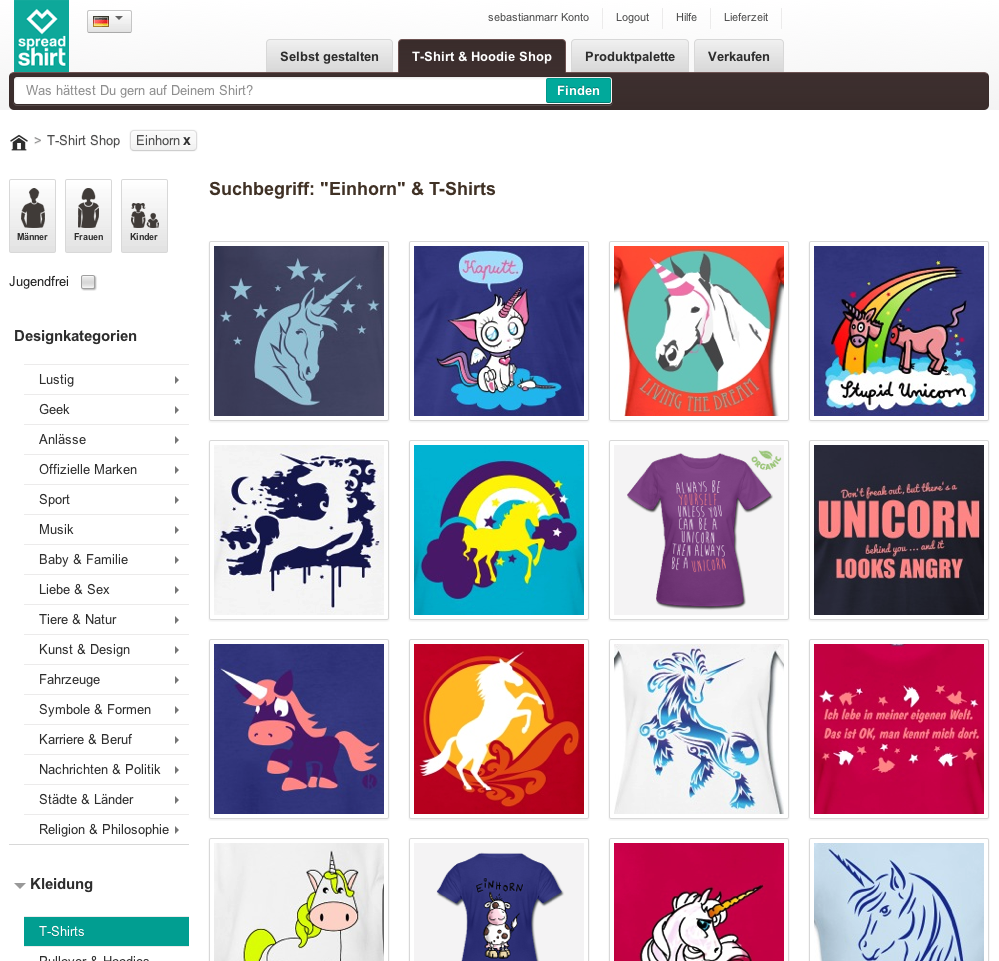
\includegraphics[width=0.9\textwidth]{search_result}
\caption{Suchergebnisseite}
\label{fig:search_result}
\end{figure}

Aufgrund der kürzlichen Einführung des Clicktracking-Systems wurde im Kontext dieser Arbeit mit den ersten \num{611836} aufgezeichneten Klicks gearbeitet.

\subsection{Datenqualität}

Die Qualität von Daten wird im Allgemeinen unter mehreren Gesichtspunkten beurteilt \cite{hkp2012}. Dazu gehören unter Anderem \emph{Korrektheit}, \emph{Vollständigkeit}, und \emph{Redundanzfreiheit}. Nachfolgend werden die bei Spreadshirt vorhandenen Daten nach diesen Kriterien betrachtet und die Quellen eventueller Fehler \cite[43 ff]{jo2003} diskutiert.

\paragraph{Korrektheit}

Die Korrektheit der Tag-Daten kann an vielen Punkten angezweifelt werden. Das hervorstechende Problem hierbei ist das Auftreten von Spam. Viele Partner versehen ihre Artikel und Designs mit Tags, die nicht den Inhalt beschreiben. Partner versehen ihre Designs und Artikeln mit falschen Tags, damit diese bei populären Suchbegriffen gefunden werden.

Ein weiterer Defekt ist die Inkorrektheit des Attributes \emph{Sprache} der Tags. Die Sprache wird aus der Domain abgeleitet, die der Benutzer, der den Tag eingegeben hat, besucht hat. Viele Partner geben jedoch ihre Tags in mehreren Sprachen ein, um ihre Inhalte besser auffindbar zu machen. Dies führt in der Konsequenz dazu, dass das Attribut Sprache im großen Teil der Tags als falsch angesehen werden kann.

Die Quelle beider Fehler ist also die bewusste Falscheingabe von Informationen, um einen persönlichen Vorteil zu erlangen.
                                                                                                                                                                                                                                                                                                                                                                                                              
\paragraph{Vollständigkeit}

Wie bereits in \ref{tag-system} beschrieben, fehlen in den Spreadshirt-Daten der Zeitpunkt und der Benutzer eines Taggings. Dies führt in der Konsequenz dazu, dass Spam schwerer erkannt werden kann. Zwar ist bekannt, wann ein Tag das erste Mal verwendet wurde, alle weiteren Verwendungen des Tags werden haben jedoch keinen Zeitstempel. Der Benutzer, der den Tag angelegt und verwendet hat, kann nur daraus abgeleitet werden, wer den getaggten Artikel angelegt hat.

Die Unvollständigkeit der Daten rührt in erster Linie daher, dass zum Zeitpunkt der Implementierung des Tag-Systems noch nicht bedacht wurde, dass die fehlenden Attribute später nützlich sein können.

\paragraph{Redundanzfreiheit}

Bedingt durch die Form der Dateneingabe besteht für das Vokabular des Tag-System ein großes Potential für redundante Daten. Da eingegebene Tags durch einen Separator getrennt eingegeben werden müssen, besteht hier Potential zur Fehleingabe. Wird der falsche Separator verwendet, werden die eigentlich getrennten Tags als eine einzige Entität abgespeichert.

Technisch kann jeder Tag genau ein Mal in der Datenbank vorkommen. Jedoch führen Rechtschreibfehler, unterschiedliche Groß- und Kleinschreibung, verschiedene Arten zusammengesetzte Wörter zu schreiben, Leerräume vor, nach und zwischen Wörtern eines Tags und Tippfehler dazu, dass das gleiche Wort mehrfach in der Datenbank gespeichert wurde.

Außerdem führten in der Vergangenheit Systemfehler und Implementierungsfehler dazu, dass falsche, nicht druckbare Zeichen in den Tags enthalten waren. Nach Beseitigung der Fehler blieben die fehlerhaften Tags bestehen, so dass bei einer erneuten Eingabe des gleichen Wortes ein neuer Tag in der Datenbank angelegt wurde.

\section{Lösungsansatz}

Die Beziehungen, die zwischen Wörtern und Wortgruppen hergestellt werden können, hängen stark von Umfang, Vielfältigkeit und Qualität der vorhandenen Datenquellen ab. Daher wurde zur Realisierung der Zielstellung ein iterativer Ansatz gewählt.

Die grundsätzliche Lösungsidee besteht in der Erstellung eines Graphen, dessen Knoten Wörter oder Wortgruppen darstellen. Die Kanten zwischen diesen Knoten repräsentieren inhaltliche Beziehungen. Ein erstrebenswertes Ziel ist also ein Graph mit möglichst vielen, duplikatfreien Knoten und vielen, nach inhaltlicher Nähe gewichteten, Kanten. Die hohe Knotenanzahl kommt zum Tragen, um möglichst alle Suchbegriffe und Themen des Anwendungsgebietes abzubilden. Kantenanzahl und -gewichte spielen dann eine Rolle, wenn nach den inhaltlich nächsten Nachbarn eines Knotens gesucht wird.

Um einen solchen Graphen zu erstellen, ist eine Grundmenge von Daten nötig. Diese Grundmenge stellen die Daten des Tag-Systems (\ref{tag-system}) von Spreadshirt dar. Die bereinigten Tags stellen die Knotenmenge dar. Die Kanten werden mittels Kookkurenz ermittelt.

Um die Qualität des Graphen danach schrittweise zu verbessern, werden daraufhin im Laufe der Arbeit weitere externe und interne Datenquellen integriert. Hierbei werden, soweit möglich, ebenfalls kookkurenzbasierte Ansätze gewählt. Diesem Vorgehen liegt die Annahme zu Grunde, dass oft gemeinsam auftauchende Begriffe auch eine inhaltliche Nähe zueinander aufweisen.

Bei jeder neuen Datenquelle muss zunächst die Bereinigung, Integration, Reduktion und Transformation der Daten durchgeführt werden \cite{hkp2012}. Diese Schritte gewährleisten die Datenqualität des Ergebnisgraphen.

Zusammengefasst bedeutet dies, dass abgeleitet von der vorhandenen Knotenmenge weitere Graphen aus anderen Datenquellen erstellt und diese dann in den ursprünglichen Graphen überführt werden. Dies führt einerseits unter Umständen zu einer Erweiterung der Knotenmenge und andererseits zu neuen Kanten mit neuen Gewichten.

Die gewichtete Kombination mehrerer Kanten zwischen zwei Knoten des Graphen stellt also im Ergebnis die inhaltliche Nähe der Begriffe dar, die durch die Knoten repräsentiert werden. Somit muss des weiteren eine geeignete Gewichtung der Kantentypen gefunden werden. Dies ist aufgrund der Natur des Problems nur mit Hilfe von menschlicher Bewertung möglich. Diese Optimierung kann somit gleichzeitig mit der Evaluation statt finden.

Um den Lösungsansatz technisch umzusetzen, soll wenn möglich das Programmiermodell MapReduce \cite{dg2004} eingesetzt werden, da dieses die Skalierung des Vorgehens auf beliebige Datenmengen ermöglicht. Speziell die Erstellung von Kookkurenzgraphen kann deutlich von der Verwendung dieses Verfahrens profitieren.

In den nachfolgenden Kapiteln werden die Umsetzung dieses Lösungsansatzes und die Ergebnisse detailliert beschrieben.
\chapter{Link--Discovery--Framework}

\emph{Link Discovery} \cite{na2011, vbgk2009}, oder \emph{Link Prediction} \cite{twak2003, nk2007}, bezeichnet Methoden des Data Minings \cite{hkp2012}, die zum Ziel haben, Verbindungen zwischen Objekten herzustellen. Diese Verbindungen werden aus vorhandenen Daten abgeleitet.

Das folgende Kapitel beschreibt das Framework, dass für die Link Discovery im Rahmen dieser Arbeit angewendet wurde. Das Framework beschreibt die Kombination aus dem modellierten Weltausschnitt, dem Prozess zur Herstellung der Beziehungen, Kookkurrenz als Maß für Beziehungen, Graphen als Mittel zur Beschreibung des Weltausschnittes, möglichen Datenquellen und evolutionären Algorithmen als Mittel zur Prioisierung der erzeugten Beziehungen.

\section{Modell des Weltausschnittes}
\label{world_model}

Der folgende Abschnitt beschäftigt sich mit der Modellierung des im Rahmen dieser Arbeit verwendeten Weltausschnittes. 

\begin{figure}
\centering
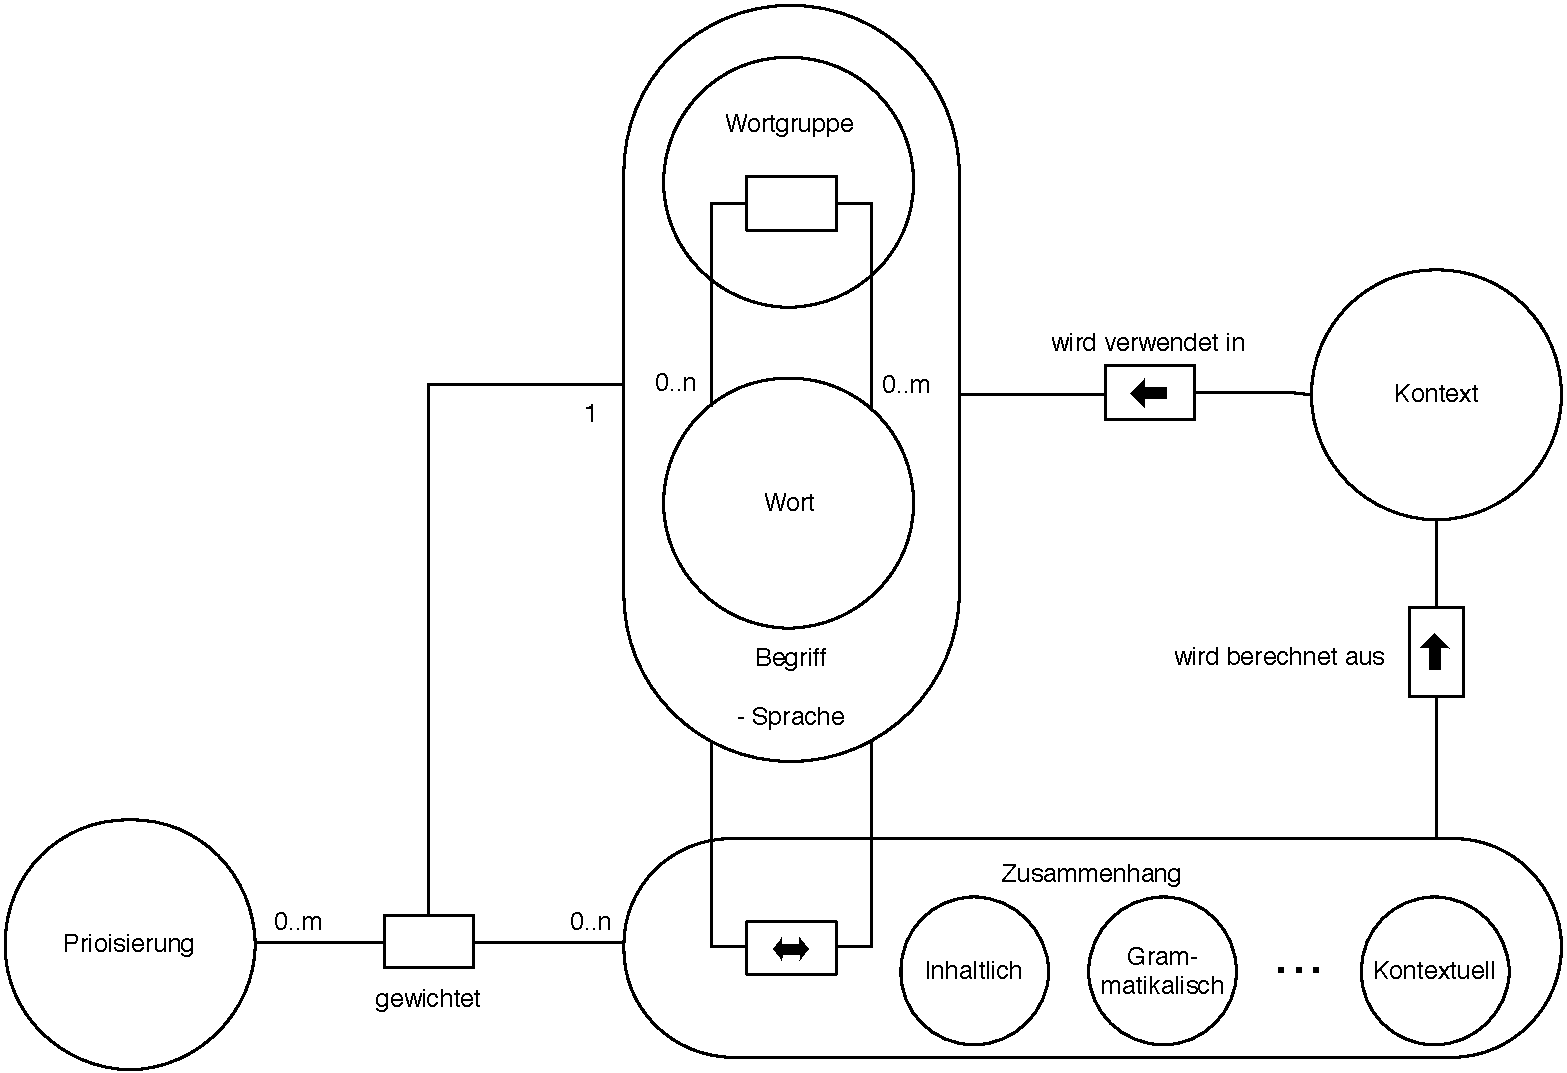
\includegraphics[width=\textwidth]{abstract_world_model}
\caption{FMC--Entity--Relationship--Diagramm des Modells des Weltausschnittes}
\label{fig:world_model}
\end{figure}

\cref{fig:world_model} zeigt das Modell als Entity--Relationship--Diagramm.

Zentrale Entität ist des Modells der \emph{Begriff}. Ein Begriff repräsentiert ein Einzelwort oder eine Wortgruppe in einer bestimmten Sprache. Dies berücksichtigt den Umstand, dass Wörter in mehreren Sprachen vorkommen können, jedoch verschiedene Bedeutungen besitzen können. Wortgruppen können aus beliebig vielen Einzelwörtern zusammengesetzt sein. Mit Hilfe der Link Discovery sollen zwischen diesen Begriffen verschiedenartige \emph{Zusammenhänge} gefunden werden.

Ein Zusammenhang besteht immer zwischen genau zwei Begriffen und besitzt einen bestimmten \emph{Typ}. Der Typ bezeichnet die Art des Zusammenhangs zwischen diesen beiden Begriffen. Beispiele für Zusammenhangsarten sind inhaltliche Zusammenhänge wie Synonyme, grammatikalische Zusammenhänge wie Wortformen und Grundformen oder kontextuelle Zusammenhänge, die sich aus der Verwendung des Begriffes ergeben. Dabei kann ein Zusammenhang abhängig vom Typ Attribute besitzen, die den Zusammenhang genauer spezifizieren. Dies kann beispielsweise ein Gewicht des Zusammenhangs sein, dass die Wichtigkeit gegenüber anderen Beziehungen gleichen Typs angibt.

Je nach Nutzungsform der Daten wird unter Umständen eine andere Sicht auf die Beziehungen benötigt. Eine \emph{Prioisierung} stellt eine Gewichtung der Beziehungen eines Begriffes nach Typ dar. Sie teilt jeder Zusammenhangsart ein Gewicht relativ zu den anderen Arten zu. Somit werden durch die Prioisierung bestimmte Zusammenhänge höher gewichtet als andere. Die Prioisierung wird zu einer auf den Anwendungsfall abgestimmten Ordnung der Beziehungen eines Begriffes genutzt.

Dies Verwendung eines Begriffes wird durch den \emph{Kontext} beschrieben. Dieser Kontext repräsentiert, \emph{wo}, \emph{wie} und \emph{wann} der Begriff innerhalb einer bestimmten Anwendungsdomäne verwendet wurde. Daher sind die Attribute, die ein Kontext besitzen kann, nicht vorab spezifizierbar. Sie hängen von der jeweiligen Anwendungsdomäne ab. Beispiele für Kontexte sind die Verwendung eines Begriffes in einem Tag--System oder in einer Ontologie.

Dieses Modell bildet die Grundlage für  im folgenden Abschnitt beschriebenen Link--Discovery--Prozess.

\section{Link--Discovery--Prozess}
\label{ld_process}

Der Link--Discovery--Prozess beschreibt die Abfolge von Schritten, die zur Erzeugung und Anreicherung des in \cref{world_model} beschriebenen Weltausschnittes angewendet werden. Dieser Prozess dient also zur Erzeugung von Begriffen und deren Zusammenhängen. \cref{fig:link_discovery_process} zeigt den Prozess als Petri--Netz.

\begin{figure}
\centering
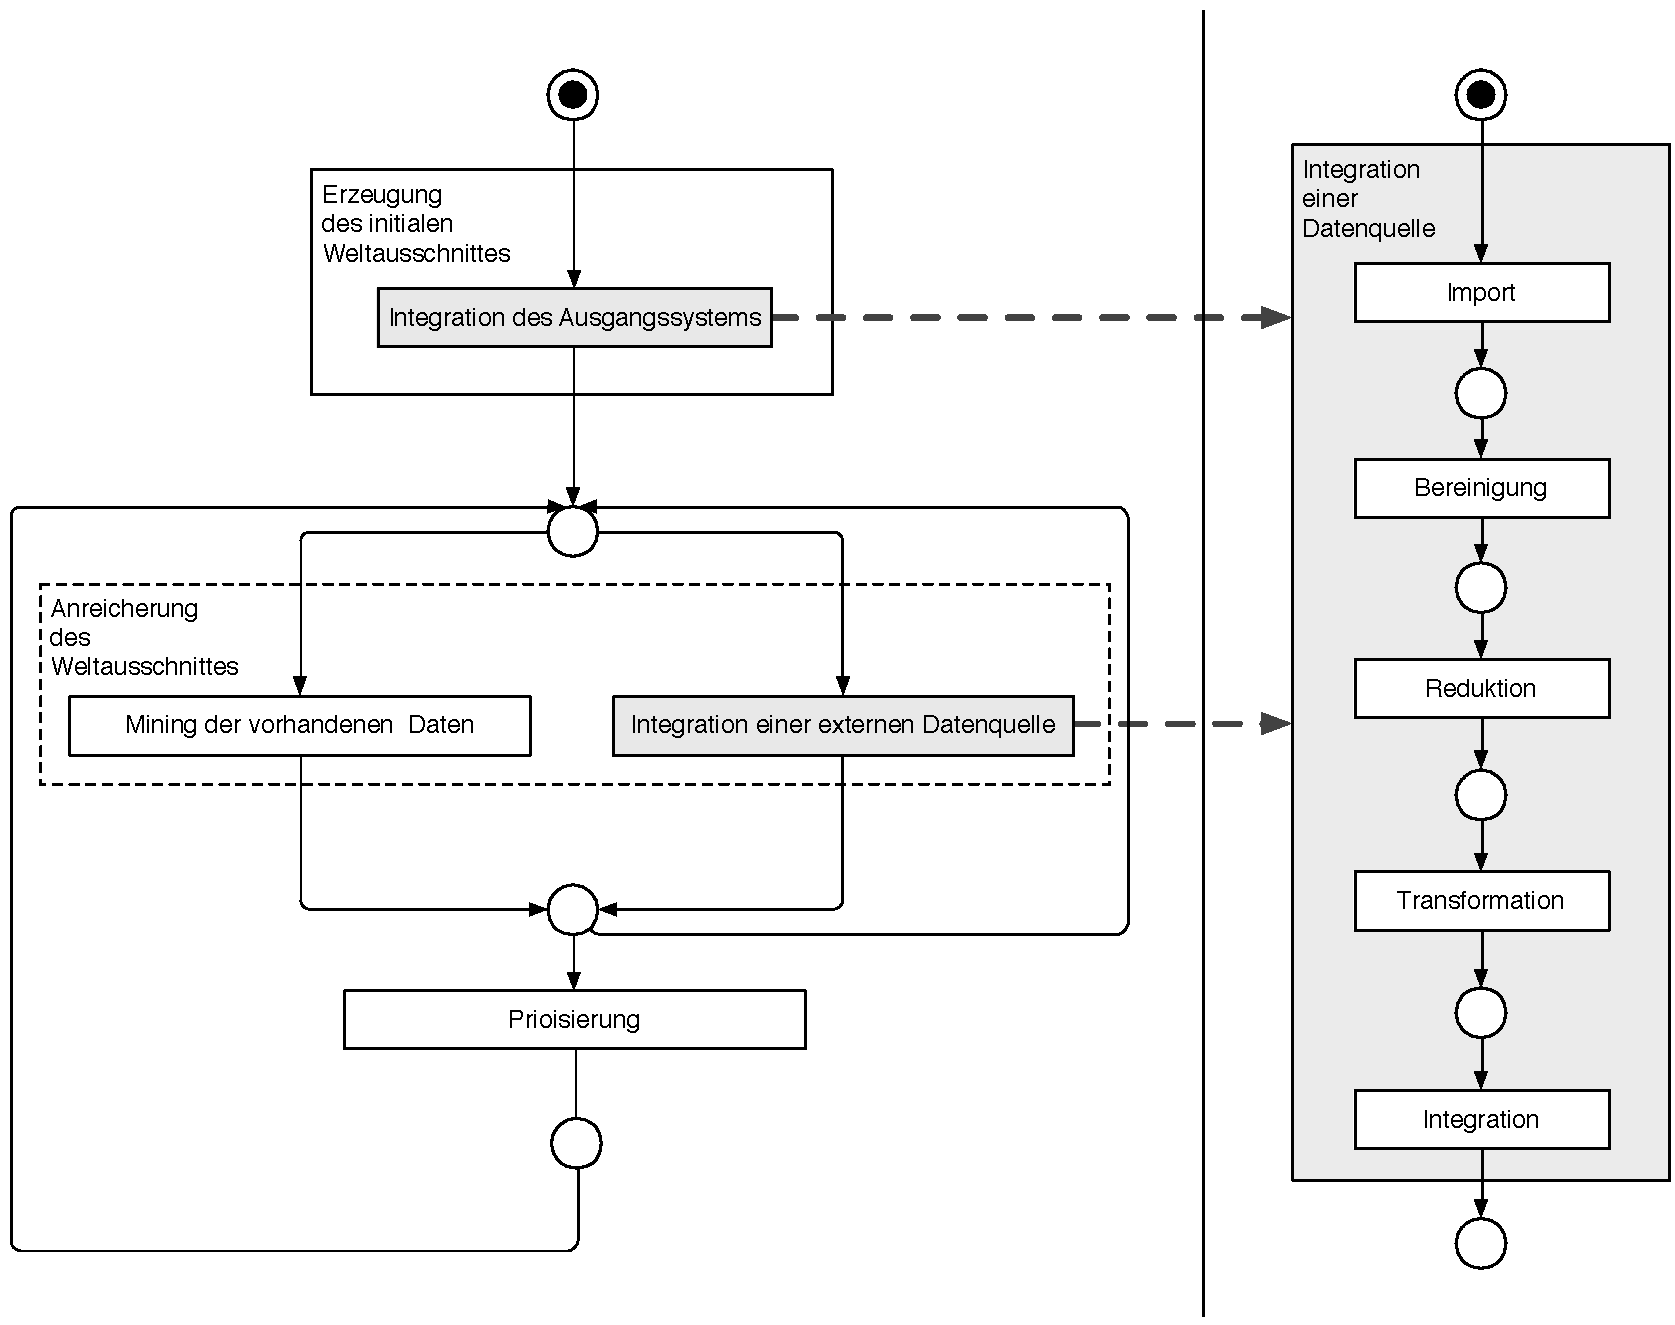
\includegraphics[width=\textwidth]{link_discovery_process}
\caption{FMC--Petri--Netz des Link--Discovery--Prozesses}
\label{fig:link_discovery_process}
\end{figure}

Die grundlegenden Phasen des Prozesses sind die \emph{Erzeugung} des initialen Weltausschnittes, dessen \emph{Anreicherung} und die \emph{Prioisierung} der Beziehungen. Sowohl bei der initialen Erzeugung, als auch bei der Anreicherung wird ein Prozess zur Integration von Datenquellen benötigt.

Die Schritte der Anreicherung und Prioisierung können beliebig oft wiederholt werden, um das Ergebnis zu verbessern und auf die gewünschte Anwendung anzupassen. Die Anreicherung kann grundsätzlich durch das Mining der bereits im Weltausschnitt vorhandenen Daten oder durch die Integration neuer Datenquellen erfolgen.

Die genannten Schritte werden in den folgenden Abschnitten erläutert.

\subsection{Integration von Datenquellen}
\label{integration_generic}

Für die Link Discovery wird ein einheitliches Vorgehen zur Integration von Datenquellen benötigt. Die Datenquellen stellen grundsätzlich für die Link Discovery nützliche Daten zur Verfügung, die jedoch im Allgemeinen noch nicht direkt dem Modell des Weltausschnittes entsprechen. Demzufolge müssen diese Daten entsprechend vorverarbeitet werden.

Die zur Integration von externen Datenquellen nötigen Schritte entsprechen im Wesentlichen den von \textcite[S. 48f.]{hkp2012} beschriebenen Aufgaben der Datenvorverarbeitung: \emph{Bereinigung}, \emph{Reduktion}, \emph{Transformation} und \emph{Integration}. Diesen wird in dieser Arbeit der Schritt \emph{Import} vorangestellt, da es nicht immer möglich ist, den gesamten Datenbestand einer Datenquelle zu nutzen. Somit sollten im Importschritt auch die Anfragen an die Datenquelle spezifiziert werden. Die genannten Schritte werden zur Link Discovery immer in der genannten Reihenfolge ausgeführt und werden im folgenden kurz beschrieben.

\paragraph{Import}

Im Importschritt werden die Rohdaten aus der Datenquelle extrahiert. Dabei wird die Form der Daten nicht verändert. Ist es nicht möglich, den gesamten Datenbestand einer Quelle zu importieren, so muss eine Auswahl der anzufragenden Daten formuliert werden. Diese Auswahl richtet sich nach Möglichkeit nach den bereits im Weltausschnitt vorhandenen Daten.

\paragraph{Bereinigung}

Im nachfolgenden Bereinigungsschritt werden die importierten Daten so gut wie möglich von eventuell vorhandenen Defekten bezüglich der Datenqualität (siehe auch \cref{quality}) befreit. Dazu zählen beispielsweise das Entfernen nicht nutzbarer Zeichen oder von unvollständigen Datensätzen.

\paragraph{Reduktion}

Der Reduktionsschritt dient zur Verkleinerung der Datenmenge. Dazu gehören beispielsweise Schritte zur Duplikatentfernung oder zur Auswahl relevanter Datensätze. In dieser Arbeit bestand die Haupteinschränkung der Datenmenge darin, nach Möglichkeit nur deutschsprachige Datensätze auszuwählen.

\paragraph{Transformation}
\label{transformation}

Der Schritt der Transformation überführt die Daten schließlich in das Modell des Weltausschnittes. Dies bedeutet, dass die Datensätze in Begriffe und Beziehungen umgewandelt werden. Dabei sollten so viele Informationen über den Kontext der Begriffe erhalten bleiben. Die Methode, wie diese Transformation vorgenommen wird, hängt von der Datenquelle ab. Generell werden die Beziehungen meist aus dem Kontext der Begriffe, wie er in der Datenquelle vorliegt, gebildet. Ein Mittel für die Beziehungserzeugung ist die Kookkurrenz, welche in \cref{co-occurence} erläutert wird. Somit stellt der Transformationsschritt die wichtigste Komponente für die Integration einer Datenquelle dar.

\paragraph{Integration}

Der Integrationsschritt für jede Datenquelle dient letztendlich der Zusammenführung des im Transformationsschritt erzeugten Weltausschnittes mit dem bereits vorhandenen Weltausschnitt. Dabei werden bereits existierende Begriffe zusammengeführt und die neu erzeugten Beziehungen übernommen. Die Zusammenführung der Begriffe erfolgt über die Annotation des existierenden Begriffes mit dem neu erzeugten Kontext, den die Datenquelle zu einem Begriff liefert.

\subsection{Initiale Erzeugung des Weltausschnittes}

Der erste Schritt der Link Discovery besteht in der Auswahl einer geeigneten Datenquelle für die initiale Erzeugung des Weltausschnittes. In dieser Arbeit ist diese Datenquelle das Tagging--System von Spreadshirt (siehe \cref{tag_sprd}).

Die Auswahl der Datenquelle richtet sich im wesentlichen danach, ob der Kontext, den die Datenquelle potentiell zu Begriffen liefern kann, für die Link Discovery geeignet ist. Der Kontext sollte außerdem für die geplante Anwendung der Link--Discovery--Ergebnisse relevant sein.

Nach der Auswahl einer geeigneten Quelle werden die in \cref{integration_generic} beschriebenen Schritte zur Integration durchgeführt. Der letzte Schritt ist trivial, da zu diesem Zeitpunkt noch keine Daten im Weltausschnitt vorhanden sind.

\subsection{Anreicherung des Weltausschnittes}

Nach der initialen Erzeugung des Weltausschnittes kann dieser mit beliebig vielen Anreicherungsschritten ergänzt werden. Unter Anreicherung wird die Erzeugung neuer Begriffe, Kontexte oder Zusammenhänge verstanden.

Das Hinzufügen neuer Begriffe erweitert das Vokabular des Weltausschnittes. Somit können bei der Benutzung der Daten zu einer größeren Menge von Begriffen Zusammenhänge gefunden werden. Die Erzeugung von Kontexten zu vorhandenen oder neuen Begriffen erweitert das Wissen über die Benutzung eines Begriffes innerhalb einer bestimmten Anwendungsdomäne. Die Anreicherung des Weltausschnittes mit neuen Zusammenhängen ermöglicht einerseits das Finden von relevanten Nachbarn eines Begriffes, erfordert andererseits jedoch, abhängig von der Anwendung, auch eine andere Prioisierung der Zusammenhangstypen bei der Abfrage.

Grundsätzlich kann die Anreicherung des Weltausschnittes auf zwei Arten erfolgen. Dies ist zum die Anreicherung durch das Mining der bereits vorhandenen Daten, zum anderen die Anreicherung durch Integration einer weiteren Datenquelle.

\subsubsection{Anreicherung durch Mining vorhandener Daten}

Die Erzeugung neuer Begriffe und Zusammenhänge kann aus den vorhandenen Daten mittels Methoden des Data Minings vorgenommen werden. Dazu werden die bereits im Weltausschnitt vorhandenen Begriffe mit ihren Kontexten und Beziehungen analysiert, um bisher unbekannte Zusammenhänge zu finden.

Beispiele für anwendbare Methoden sind hierbei Assoziationsanalyse \cite[S. 328f.]{pt2013} oder Clusteranalyse \cite[S. 443f.]{hkp2012}, um bestimmte bereits in den Daten vorhandene, aber nicht explizit abgebildete, Zusammenhänge zu ermitteln. Jedoch können auch einfachere Methoden wie die Zerlegung von Wortgruppen in Einzelwörter (siehe \cref{decomposition}) oder das Einfügen von bisher nur transitiv vorhandenen Beziehungen erfolgreich sein, um neue Begriffe und Beziehungen in den Datenbestand einzuführen.

\subsubsection{Anreicherung durch Integration externer Datenquellen}

Sofern weitere Datenquellen verfügbar sind, stellt die Integration dieser einen weiteren erfolgversprechenden Weg dar, um die Daten anzureichern. Neue Datenquellen beschreiben immer einen neuen Kontext, in dem Begriffe genutzt werden. Ist der Kontext dieser Begriffe für die spätere Anwendung relevant, ist die Integration der jeweiligen Datenquelle zu Zwecken der Link Discovery von großem Interesse.

Um die zusätzliche Datenquelle zur Link Discovery zu nutzen, werden die gleichen Schritte, die schon zur initialen Erzeugung des Weltausschnittes zum Einsatz kamen, genutzt (siehe \cref{integration_generic}). Dazu werden im Transformationsschritt Daten erzeugt, die dem Modell des Weltausschnittes entsprechen. Im Integrationsschritt werden sie mit den bereits vorhandenen Daten zusammengeführt.

\subsection{Prioisierung von Beziehungen}

Ziel des Prioisierungsschrittes der Link Discovery ist das Finden einer Gewichtung der Zusammenhangstypen, die für einen Anwendungsfall relevante Nachbarn zu einem Begriff liefert. Die Relevanz kann jedoch nur von einem Benutzer bewertet werden. \cref{fig:prioritization} stellt den Prioisierungsprozess dar.

\begin{figure}
\centering
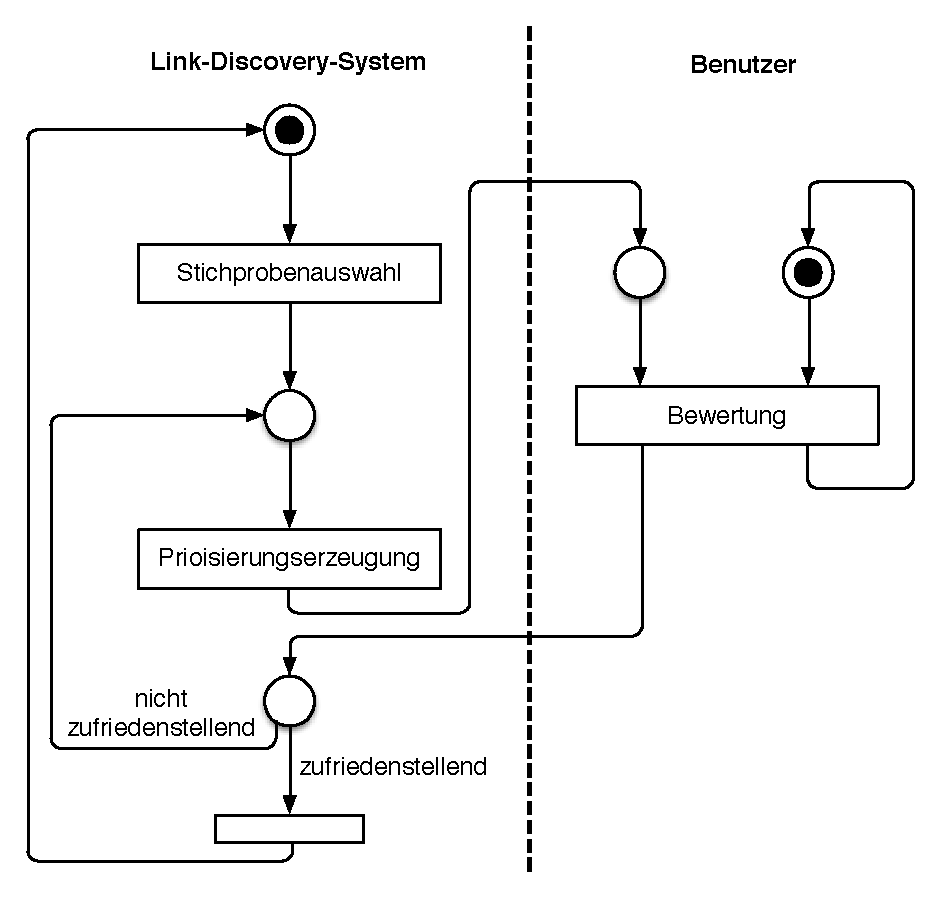
\includegraphics[width=0.7\textwidth]{prioritization}
\caption{FMC--Petri--Netz der Prioisierung}
\label{fig:prioritization}
\end{figure}

Grundsätzlich kann nicht davon ausgegangen werden, dass eine Prioisierung für alle im Weltausschnitt gespeicherten Begriffe relevante Nachbarn liefert. Daher sollte die Prioisierung stichprobenhaft für einzelne Begriffe durchgeführt werden, um dann möglicherweise eine global gute Ergebnisse liefernde Prioisierung zu ermitteln.

Der Prioisierungsprozess beginnt mit der Auswahl einer Stichprobe anhand geeigneter Kriterien für das Anwendungsszenario. Beispielhaft für Kriterien sind externe Faktoren wie die Popularität des Begriffes in der Anwendungsdomäne oder im Weltausschnitt gespeicherte Faktoren wie die Anzahl der Zusammenhänge eines Begriffes. Wird der Prozess mit mehreren Stichprobe durchgeführt, sollte auf eine möglichst breite Streuung des jeweiligen Kriteriums geachtet werden, um die Güte der Prioisierungen abhängig vom Begriff beurteilen zu können.

Nach der Auswahl der Stichprobe wird vom Link--Discovery--System eine Prioisierung erzeugt. Wie diese Erzeugung konkret implementiert ist, hängt von der Anwendung ab. Im Rahmen dieser Arbeit wurden Evolutionäre Algorithmen (siehe \cref{evo}) gewählt. Die erzeugte Prioisierung wird auf den Begriff angewandt und von einem Benutzer bewertet. Der Benutzer sollte Wissen über die Anwendungsdomäne besitzen.

Ist die Bewertung der Prioisierung positiv, ist der Prioisierungsprozess beendet. Bei nicht zufriedenstellendem Ergebnis wird die Erzeugung einer neuen Prioisierung und die anschließende Bewertung wiederholt. Stellt sich auch nach einer im Voraus gewählten Anzahl von Iterationen dieser Art kein zufriedendstellendes Ergebnis ein, so sollte die Prioisierung abgebrochen werden und die Gründe für das Fehlschlagen analysiert werden. Diese können beispielsweise in einer schlechten Qualität der Beziehungen des Weltausschnittes, in einer unpassenden Stichprobenauswahl oder fehlendem Wissen des Benutzers gefunden werden.

\section{Kookkurrenz als Mittel zur Beziehungserzeugung}
\label{co-occurence}

Im Transformationsschritt der Link Discovery (\cref{transformation}) wird eine Methode benötigt, aus dem Kontext von Begriffen Beziehungen zwischen eben jenen zu berechnen. Eine der möglichen Methoden ist die Berechnung von \emph{Kookkurrenz}. Diese wird im folgenden Abschnitt näher erläutert.

\subsection{Grundlagen von Kookkurrenz}

Um gewichtete inhaltliche Beziehungen zwischen Begriffen herstellen zu können, wird eine Definition von \emph{Ähnlichkeit} benötigt. Diese lässt sich auf vielfältige Arten bestimmen.

Die Ähnlichkeit zwischen zwei Dokumenten kann grundsätzlich nach \textcite{at1977} definiert werden. Dieser Definition liegt zu Grunde, dass sich die Dokumente als Mengen von Eigenschaften beschreiben lassen. Im Gegensatz zu anderen Ähnlichkeitsmodellen hängt die Ähnlichkeit nicht nur von den gemeinsamen Eigenschaften der Dokumente ab, sondern auch von den Eigenschaften, die die Dokumente allein besitzen. Diese Definition von Ähnlichkeit wird in \cref{fig:similarity} veranschaulicht.

\begin{figure}
\centering
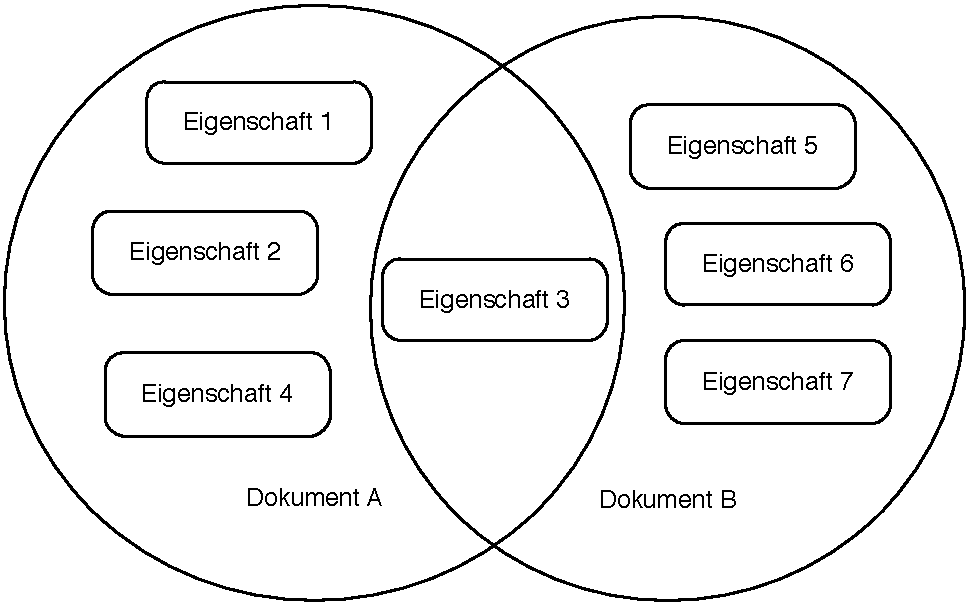
\includegraphics[width=0.6\textwidth]{similarity}
\caption{Repräsentation von Dokumenten als Mengen von Eigenschaften}
\label{fig:similarity}
\end{figure}

Somit lässt sich Ähnlichkeit \(s(A,B)\) zwischen den Dokumenten, die durch die Mengen \(A\) und \(B\) dargestellt werden, definieren durch
\[s(A,B) = F(A \cap B, A-B, B-A)\]
\label{similarity}

Die Gestaltung der Funktion \(s\) und die Auswahl der für die Ähnlichkeitsberechnung genutzten Eigenschaften der Dokumente hängt stark von der Anwendung ab. Somit beschreibt beispielsweise die Levenshtein--Distanz \cite{vl1966} die Ähnlichkeit zweier Zeichenketten durch die minimale Menge von Einfüge-, Lösch- und Ersetzungsoperationen, die nötig sind, um eine Zeichenkette in die andere umzuwandeln. In Ontologien und Taxonomien kann die Ähnlichkeit von Begriffen mittels der Knoten- oder Kanteneigenschaften berechnet werden. Beispiele hierfür sind die Ähnlichkeit in Ontologien nach \textcite{pr1995} und \textcite{ps2002}. In der Bildverarbeitung können merkmalsbasierte Ähnlichkeitsmaße ebenfalls eingesetzt werden, beispielsweise beschreiben \textcite{ow2006} ein Ähnlichkeitsmaß auf Basis von Clusteringalgorithmen, die auf Rastergrafiken angewandt werden.

Im Rahmen dieser Arbeit wird ein Ähnlichkeitsmaß gesucht, dass anhand der Eigenschaften von Begriffen eine Distanz zwischen eben jenen berechnet. Da eine inhaltliche Ähnlichkeit gesucht wird, spielen linguistische Ähnlichkeitsmaße wie die Levenshtein--Distanz eine untergeordnete Rolle. Zu Beginn bestehen keinerlei Verbindungen zwischen den Begriffen, so dass keine Ähnlichkeitsmaße für Ontologien eingesetzt werden können. Somit bietet sich die Wahl eines Ähnlichkeitsmaßes an, das den Kontext, in dem die Begriffe im Quellsystem verwendet werden, berücksichtigt.

In \cref{data} wurde das für diese Arbeit verfügbare Tagging--System beschrieben. In diesem System besitzen die Tags wenig Kontext. Die einzig verfügbare Information ist, an welche Dokumente die Tags vergeben wurden.

Wenn mehrere Begriffe pro Dokument verwendet werden, wird damit ein Zusammenhang zwischen den Begriffen beschrieben. Dieser Zusammenhang lässt sich mit dem Ähnlichkeitsmaß \emph{Kookkurrenz} messen. Kookkurrenzmaße beschreiben, wie oft Begriffe gemeinsam verwendet werden. Dies wird ins Verhältnis zum einzelnen Auftreten der Begriffe gesetzt und genügt somit der Definition von Ähnlichkeit in \cref{similarity}.

Hierzu muss angemerkt werden, dass die Ähnlichkeit mittels Kookkurrenz nicht zwingend eine Ähnlichkeit der den Begriffen zu Grunde liegenden Konzepte darstellt. Die Verwendung von Kookkurrenz als Ähnlichkeitsmaß beruht allein auf der Annahme, dass Menschen zur Beschreibung von gleichen Inhalten die gleichen Begriffe benutzen. Diese Annahme muss im Laufe der Evaluierung der Ergebnisse validiert werden.

\subsection{Kookkurrenzmaße}
\label{measures}

Werden die Objekte, zwischen denen die Ähnlichkeit berechnet werden soll, als Mengen von Eigenschaften definiert, bieten sich die üblichen Kennzahlen für die Ähnlichkeiten von Mengen an. Ein Begriff kann also als Menge der Dokumente, für die er als Beschreibung verwendet wurde, definiert werden.

Um die Ähnlichkeit zwischen zwei Begriffen zu ermitteln, lassen sich die Vereinigungsmenge, Schnittmenge und Kreuzprodukte der jeweiligen Mengen bilden, die die Begriffe repräsentieren. Ist also \(A\) die Menge der Dokumente, die mit einem Begriff \(a\) versehen wurden, \(B\) die Menge der Dokumente mit einem Begriff \(b\), so ergeben sich die Mengen:

\begin{itemize}
    \item \(A \cap B\), alle Dokumente die mit \(a\) und \(b\) versehen wurden
    \item \(A \cup B\), alle Dokumente die mit \(a\) oder \(b\) versehen wurden
    \item \(A \times B\), alle Dokumentenpaare, die sich aus den Mengen \(A\) und \(B\) bilden lassen
\end{itemize}

Die Mächtigkeiten dieser Mengen können dann zur Berechnung verschiedener Ähnlichkeitsmaße verwendet werden. Drei der üblichsten Maße wurden im Rahmen dieser Arbeit verwendet und werden im Folgenden genannt.

\subsubsection{Sørensen--Dice}

Der Sørensen--Dice--Koeffizient \cite{st1948} \cite{ld1945}, oft auch nur Dice--Koeffizient, enstand ursprünglich in der Biologie und wurde verwendet, um die Ähnlichkeit zwischen Proben zu berechnen. Heute findet er allgemeine Anwendung im Data Mining. Er ist definiert durch:

\[
\delta_{Dice}(a, b) = \frac{2|A \cap B|}{|A|+|B|}
\]

Der Wertebereich des Koeffizienten liegt zwischen \num{0} und \num{1}.

\subsubsection{Jaccard}

Der Jaccard--Index \cite{pj19012} wurde ursprünglich mit dem gleichen Zweck wie der Dice--Koeffizient verwendet. Sein Wertebereich liegt ebenfalls zwischen \num{0} und \num{1} und er ist definiert durch:

\[
\delta_{Jaccard}(a,b) = \frac{|A \cap B|}{|A \cup B|}
\]

\subsubsection{Kosinus}

Die Kosinus-Ähnlichkeit \cite{hkp2012} ist ursprünglich ein Maß für die Ähnlichkeit zweier Vektoren. Sie ist eine Maßzahl dafür, ob die Vektoren ungefähr in die gleiche Richtung zeigen. Sie kann jedoch genauso auf Mengen angewendet werden, da das Vorhandensein der Elemente in der Menge auch durch einen Vektor in einem \(n\)-dimensionalen Raum dargestellt werden kann, wobei \(n\) die Anzahl aller möglichen Eigenschaften ist. Der Wertebereich der Kosinus-Ähnlichkeit liegt ebenfalls zwischen \num{0} und \num{1}. Sie ist auf den in \cref{measures} definierten Mengen definiert durch:

\[
\delta_{Cosine}(a, b) = \frac{|A \cap B|}{\sqrt{|A| \times |B|}}
\]

Nachdem die Ähnlichkeit mittels Kookkurrenz und die entsprechenden Maße vorgestellt wurden, wird im nächsten Abschnitt die Berechnung und damit verbundene Komplexität diskutiert.

\subsection{Berechnung von Kookkurrenz}

Um die in \cref{measures} genannten Maße für Kookkurrenz zu berechnen, muss das Kreuzprodukt aller Begriffe gebildet werden. Dabei muss für jedes Paar von Begriffen die Häufigkeit gezählt werden, wie oft die Begriffe gemeinsam zur Verschlagwortung von Dokumenten verwendet wurden. Diese Häufigkeit beschreibt die Mächtigkeit der Mengen \(A \cap B\). Außerdem muss gezählt werden, wie oft jeder Begriff insgesamt verwendet wird, um die Mächtigkeit der Mengen \(A, B, \dots\) zu bestimmen. Danach können über die genannten Formeln die Kookkurrenzmaße berechnet werden. In \cref{lst:coocc-pseudo} ist die Berechnung als Pseudo--Code dargestellt.

\begin{lstlisting}[language=pseudo, label={lst:coocc-pseudo}, caption={Kookkurrenzberechnung}]
var occurences = {};

foreach (term in terms) {
    occurences[term] = countOccurrences(term);
}

foreach (termA in terms) {
    foreach (termB in terms) {
        ab = countCoOccurences(termA, termB);
    }
    dice = dice(occurences[termA], occurences[termB], ab);
    jaccard = jaccard(occurences[termA], occurences[termB], ab);
    cosine = cosine(occurences[termA], occurences[termB], ab);
}
\end{lstlisting}

Der Aufwand, um die Kookkurrenzmaße für alle Paare von Begriffen zu berechnen, hängt also von der Anzahl der Begriffe, Dokumente und Verwendungen ab. Beträgt die Anzahl der Begriffe \(n\) und die Anzahl der Dokumente \(d\), so ergibt sich für den Fall, dass jeder Begriff an jedes Dokument vergeben wurde eine Laufzeit von \(O(d*n^2)\). Wurden keine Begriffe mit Dokumenten verknüpft, beträgt die Laufzeit \(\Theta(d)\). Die reale Laufzeit der Ähnlichkeitsberechnung liegt daher zwischen diesen Schranken.

Es ist also absehbar, dass der Rechenaufwand mit wachsender Datenmenge stark ansteigt. Somit scheint es ratsam, nach Optimierungen zu suchen, um die Rechenzeit zu verringern. Da sich die Anzahl der Berechnungen nicht vermindern lässt, kann eine Verkürzung der Rechenzeit nur durch Parallelisierung erreicht werden. Eine mögliche Umsetzung der parallelen Berechnung der Kookkurrenz mittels des MapReduce--Programmiermodelles wird in \cref{mapreduce_cooccurence} erläutert.

\section{Graphen als Beschreibungsmittel des Weltausschnittes}

Nachdem in \cref{world_model} der zur Link Discovery verwendete Weltausschnitt modelliert wurde, wird zur Umsetzung eine Datenstruktur benötigt, die diesen Ausschnit konkret abbildet. Da im Wesentlichen Objekte, ziwschen denen Verbindungen bestehen, abgebildet werden, bietet sich die Verwendung eines Graphen an. Die Grundlagen von Graphen, sowie die konkrete Abbildung des Weltausschnittes auf eine Graph--Datenstruktur werden in den folgenden Abschnitten erläutert.

\subsection{Grundlagen}

Ein \emph{ungerichteter Graph} ist definiert durch ein Paar \(G = (V,E)\) von Mengen, für die gilt: \(E \subseteq\ [V]^2\). Dies bedeutet, dass alle Elemente aus \(E\) 2-elementige Teilmengen von \(V\) sind \cite[S. 2]{rd2012}. Die Menge \(V\) repräsentiert die \emph{Knoten} und die Menge \(E\) die \emph{Kanten} des Graphen. Eine Kante stellt eine Verbindung von zwei Knoten dar. Zwei Knoten werden als \emph{Nachbarn} bezeichnet, wenn zwischen ihnen eine Kante existiert. \cref{fig:basic_graph} zeigt ein Beispiel für einen ungerichteten Graphen.

\begin{figure}[h]
\centering
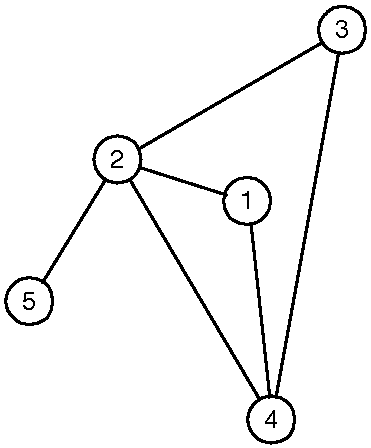
\includegraphics[width=0.2\textwidth]{basic_graph}
\caption{Ungerichteter Graph}
\label{fig:basic_graph}
\end{figure}

Ein \emph{gerichteter Graph} ist ein Graph, der neben den Mengen \(V\) und \(E\) die zwei Abbildungen \(quelle: E \rightarrow V\) und \(ziel: E \rightarrow V\) enthält \cite[S. 25]{rd2012}. Diese weisen jeder Kante \(e\) einen Quell- und Zielknoten zu. Die Kante ist somit von \(quelle(e)\) nach \(ziel(e)\) gerichtet. \cref{fig:directed_graph} zeigt einen gerichteten Graphen.

\begin{figure}[ht]
\centering
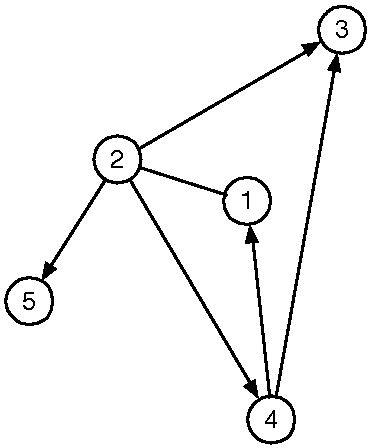
\includegraphics[width=0.2\textwidth]{directed_graph}
\caption{Gerichteter Graph}
\label{fig:directed_graph}
\end{figure}

Als \emph{Multigraph} wird schließlich ein Graph bezeichnet, bei dem zwischen zwei Knoten mehrere Kanten bestehen \cite[S. 25]{rd2012}. Sind diese gerichtet, spricht man vom einen \emph{gerichteten Multigraph}. \cref{fig:directed_multigraph} illustriert einen solchen gerichteten Multigraph.

\begin{figure}[h]
\centering
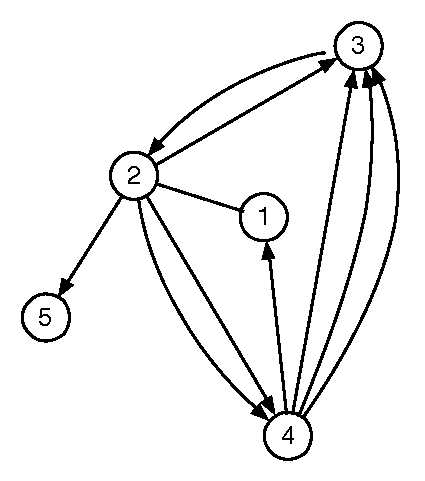
\includegraphics[width=0.2\textwidth]{directed_multigraph}
\caption{Gerichteter Multigraph}
\label{fig:directed_multigraph}
\end{figure}

Die Knoten und Kanten eines Graphen sind Objekte mit beliebigen weiteren Eigenschaften. Kanten besitzen üblicherweise ein Gewicht, dass ihre Wichtigkeit oder Kosten im Anwendungskontext des Graphen angibt.

Nachdem Graphen grundsätzlich erläutert wurden, beschäftigt sich der folgende Abschnitt mit der konkreten Umsetzung des Modelles des Weltausschnittes auf eine solche Graphen--Struktur.

\subsection{Graphenrepräsentation des Weltausschnittes}

\section{Datenquellen zur Anreicherung}

\section{Evolutionäre Algorithmen als Mittel zur Prioisierung}

\section{Zusammenfassung}
\chapter{Erstellung von Kookkurrenzgraphen}

\section{MapReduce}


\section{Anwendung von MapReduce zur Kookkurrenzberechnung}


Nachdem in diesem Kapitel die theoretischen Grundlagen für die Link Discovery mittels Kookkurrenz beschrieben wurden, beschäftigt sich das folgende Kapitel mit dem technischen System zur Umsetzung des Lösungsansatzes.
\chapter{Systembeschreibung}
\label{system}

Das nachfolgende Kapitel befasst sich mit der Beschreibung der Technologien und Vorgehensweisen, die zur Link Discovery im Rahmen dieser Arbeit angewendet wurden. Dazu zählen im Einzelnen die gewählte Datenbank MongoDB, das Datenmodell des Zielgraphen und das daraus resultierende Vorgehen und die Architektur des Systems zur Link Discovery.

\section{MongoDB}
\label{mongo}

Zur Umsetzung der Link Discovery wurde das Datenbankmanagementsystem MongoDB \cite{mo2013} gewählt. Bei MongoDB handelt es sich um eine quelloffene dokumentenorientierte Datenbank.

Im Gegensatz zu traditionellen relationalen Datenbanksystemen verzichtet MongoDB dabei auf eine tabellenförmige Struktur der Daten und speichert Datensätze in Form von so genannten \emph{Dokumenten}. Dabei handelt es sich um hierarchische Schlüssel-/Wertpaare, die schemalos in so genannten \emph{Collections} gespeichert werden. Schemalos bedeutet dabei, dass die Dokumente innerhalb einer Collection nicht alle dieselbe Struktur besitzen müssen.

Zur Repräsentation der Dokumente verwendet MongoDB ein Format, dass sich sehr an JSON \cite{json2006} anlehnt. JSON ist ein menschenlesbares Datenaustauschformat, das aus der Objektnotation der Programmiersprache JavaScript abgeleitet wurde. Das Datenformat von MongoDB ist BSON \cite{bson2013}, eine binäre Repräsentation von JSON, die einige zusätzliche Datentypen unterstützt. 

Listing \ref{lst:json} zeigt ein Beispiel für ein Dokument in MongoDB. Das Feld \emph{\_id} ist hierbei ein  Bezeichner vom Typ \emph{ObjectID}. Dieser stellt einen global eindeutigen Bezeichner dar, der benutzt werden kann, um Dokumente zu referenzieren. Innerhalb einer Collection ist \emph{\_id} dabei grundsätzlich eindeutig. Das Feld \emph{address} zeigt, dass Dokumente weitere Dokumente enthalten können. Das Feld \emph{friends} zeigt, dass Werte für Schlüssel auch Arrays von Werten sein können. Diese sind dabei nicht auf primitive Typen wie Zeichenketten oder Zahlen beschränkt, sondern können auch weitere Dokumente sein.

\begin{lstlisting}[language=json, label={lst:json}, caption={Ein Beispiel für ein Dokument in MongoDB}]
{
    "_id" : ObjectId("51efc20147cae77dfc02e0ac"),
    "name" : "Bob",
    "age": 25,
    "address": {
        "city": "Leipzig",
        "street": "Karl-Liebknecht-Str. 132"
        "zip": "04277"
    },
    "friends" : [
        "alice",
        "fred",
        "jason"
    ]
}
\end{lstlisting}

MongoDB unterstützt Anfragen über ein Binärprotokoll, welches über so genannte \emph{Treiber} in vielen Programmiersprachen abstrahiert zur Verfügung steht. Dabei sind vielfältige Lese- und Schreiboperationen möglich, die komplexe Abfragen und Operationen auf den gespeicherten Daten zulassen. Außerdem bietet MongoDB eine Implementierung des MapReduce-Programmiermodells (siehe \ref{mapreduce}) sowie die Möglichkeit, Indizes auf allen Hierarchieebenen der Dokumente zu nutzen. Für interaktive Operationen steht die \emph{Mongo Shell} zur Verfügung, welche Abfragen mittels der Programmiersprache JavaScript erlaubt und somit einen Treiber für diese Sprache darstellt.

Aufgrund der genannten Eigenschaften stellt MongoDB einen exzellenten Ausgangspunkt für die Link Discovery im Rahmen dieser Arbeit dar. Durch die vorhandene Schemaflexibilität können die Daten in der gerade benötigten Form gespeichert und abgefragt werden. Durch die Unterstützung von MapReduce mit mehreren Rechnern lassen sich Berechnungen wie die der Kookkurrenz (siehe \ref{mapreduce_cooccurence}) parallelisieren und somit beschleunigen.

Aus diesen Gründen stellt MongoDB das zentrale technische Element für die Link Discovery im Rahmen dieser Arbeit dar. Sobald die Daten aus den externen und internen Quellen in MongoDB importiert wurden, können die folgenden Schritte direkt mit Datenbankabfragen realisiert werden.

\section{Datenmodell}

Nach der Auswahl eines geeigneten Datenbanksystems sollte das Datenmodell des Ergebnisses genauer spezifiziert werden. Ist dieses vor der Link Discovery klar, können die einzelnen benötigten Schritte zur Erreichung des Zieles einfacher definiert werden.

Generell handelt es sich bei dem gewünschten Ergebnis um einen gerichteten Multigraph. Dieser repräsentiert Objekte, oder auch \emph{Knoten}, zwischen denen paarweise Verbindungen, die \emph{Kanten} bestehen. Die Besonderheit eines Multigraphen ist dabei, dass zwischen zwei Knoten auch mehrere Kanten existieren dürfen \cite{rd2012}. Dies ist dem gewählten Lösungsansatz geschuldet, da zwischen Wörtern und Wortgruppen verschiedenartige Beziehungen existieren können.

Somit müssen für das Datenmodell die beiden Entitäten \emph{Knoten} und \emph{Kante} modelliert werden.
Das komplette Datenmodell des Graphen nach der Integration aller Datenquellen ist in Anhang \ref{complete_data_model} dargestellt.

\subsection{Knoten}

Die Knoten repräsentierendie Wörter und Wortgruppen zwischen denen durch Link Discovery Verbindungen hergestellt werden sollen. Sie enthalten als benötigte Attribute eine Zeichenkette und ein Attribut Sprache. Die Kombination dieser beiden Attribute ist innerhalb der Knotenmenge eindeutig. Außerdem erhält jeder Knoten zur einfacheren Referenzierung einen eindeutigen Bezeichner.

Neben diesen immer vorhandenen Attributen kann ein Knoten beliebig viele weitere Eigenschaften besitzen. Diese Eigenschaften dienen dazu, den Begriffen, die die Knoten existieren, für spätere Verwendungen zusätzlichen Kontext zu geben. Im Wesentlichen definieren sich diese zusätzlichen Eigenschaften aus den Datenquellen, die zum Zweck der Link Discovery in den Graph integriert werden.

Zur besseren Kapselung und Übersicht sollten die zusätzlichen Eigenschaften in weitere Entitäten gekapselt werden. Die Struktur dieser zusätzlichen Typen kann dann zum Zeitpunkt der Integration der jeweiligen Datenquelle definiert werden.

Das resultierende Knotenmodell ist in Abbildung \ref{fig:node_erd} dargestellt.

\begin{figure}
\centering
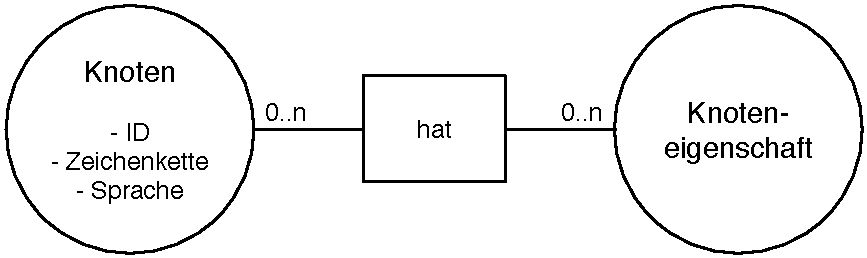
\includegraphics[width=0.6\textwidth]{node_erd}
\caption{Knotenmodell als Entity-Relationship-Diagramm}
\label{fig:node_erd}
\end{figure}

\subsection{Kanten}

Eine Kante ist im Wesentlichen durch die Knoten, die sie verbindet, beschrieben. Sie stellt einen irgendwie gearteten Zusammenhang zwischen zwei Knoten dar. Sie ist dabei gerichtet, um auch assymetrische Zusammenhänge zwischen Knoten abbilden zu können.

Somit sind die einzig immer benötigten Attribute der Quell- und Zielknoten und der Typ der Kante. Zusätzlich erhält jede Kante einen eindeutigen Bezeichner.

Alle weiteren Eigenschaften der Kante hängen vom Typ ab. Dies können beispielsweise Maße sein, die ein Kantengewicht darstellen. Da eine Kante nur genau einen Typ haben kann, werden die zusätzlichen Kanteneigenschaften einfach als Attribute an der Kante annotiert.

Das beschriebene Kantenmodell ist in Abbildung \ref{fig:edge_erd} dargestellt.

\begin{figure}
\centering
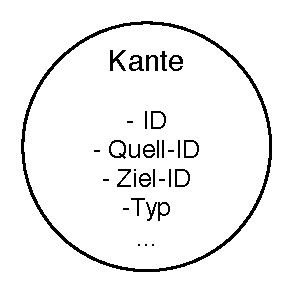
\includegraphics[width=0.2\textwidth]{edge_erd}
\caption{Kantenmodell als Entity-Relationship-Diagramm}
\label{fig:edge_erd}
\end{figure}

\subsection{Technische Umsetzung}

Um das beschriebene Datenmodell in MongoDB umzusetzen, muss es in eine Dokumentenform überführt werden. Dazu bietet sich an, Knoten in Kanten in unterschiedlichen Collections zu speichern, um sie voneinander zu trennen.

Somit stellt sich anschließend die Frage, wie die Knoten und Kanten als Dokumente repräsentiert werden. Durch die durch MongoDB gegebene Schemaflexibilität lassen sich die optionalen Eigenschaften von Knoten und Kanten direkt in den Dokumenten speichern.

Im Fall der Knoten bietet sich daher an, die zusätzlichen Eigenschaften als Unterdokumente des Knotens zu behandeln. Der Schlüssel für diese Unterdokumente ist dabei der Name der zusätzlichen Eigenschaft. Dadurch lassen sich die Knoten gut filtern, da die Abfrage auf das Vorhandensein des jeweiligen Schlüssels angepasst sein kann. Listing \ref{lst:node_json} zeigt ein Beispiel für einen Knoten in JSON-Notation. Arrays mit vielen Elementen sind dabei verkürzt dargestellt.

Die Kanten können direkt als Dokumente abgebildet werden. Über den Typ ergeben sich zusätzliche Eigenschaften. Listing \ref{lst:edge_json} zeigt beispielhaft ein Kantendokument für eine Tag-Kookkurrenz in JSON-Notation.

\begin{lstlisting}[language=json, label={lst:node_json}, caption={Knotendokument in JSON}]
{
    "_id" : ObjectId("51efc22447cae77dfc03e16b"),
    "language" : "de",
    "string" : "segeln",
    "languageDetection" : {
        "language" : "de",
        "confidence" : 1
    },
    "tagProperties" : {
        "occurenceCount" : 4678,
        "articleCount" : 2347,
        "designCount" : 2331,
        "articleIDs" : [ 
            4961057, 
            4977725, 
            ...
        ],
        "designIDs" : [ 
            1645572, 
            2216059, 
            ...
        ]
    },
    "wortschatzProperties" : {
        "synonyms" : [ 
            "flattern", 
            "fliegen", 
            "gaukeln", 
            ...
        ]
    }
}
\end{lstlisting}

\begin{lstlisting}[language=json, label={lst:edge_json}, caption={Kantendokument in JSON}]
{
        "_id" : ObjectId("51efd6f61177ff360605bd99"),
        "source" : ObjectId("51efc1af47cae77dfc00c3f8"),
        "target" : ObjectId("51efc1e047cae77dfc02087c"),
        "type" : "tag-co-occurence",
        "occurences" : 1,
        "dice" : 0.0001317089232795522,
        "jaccard" : 0.00006585879873551106,
        "cosine" : 0.008115343414514944
}
\end{lstlisting}

Nachdem die Datenformate definiert sind, beschäftigt sich das folgende Kapitel mit der Architektur des implementierten Link Discovery-Systems.

\section{Systemarchitektur}

Nach erfolgter Technologieauswahl und Modellierung der Daten soll im nächsten Abschnitt die Umsetzung der Link Discovery beschrieben werden.

Da die Mongo Shell eine vollwertige JavaScript-Laufzeitumgebung enthält und skriptbar ist, wurden die meisten Operationen im Rahmen dieser Arbeit als Skripte für diese Shell implementiert. Einzig der Import der Tag- und Clicktrackingdaten wurde mit Ruby-Skripten realisiert.

Die Schritte zur Link Discovery sind im Wesentlichen für jede zu integrierende Datenquelle gleich. Sie umfassen den Import, die Bereinigung, die Reduktion, die Transformation und die Integration der Daten \cite{hkp2012}.

\begin{figure}
\centering
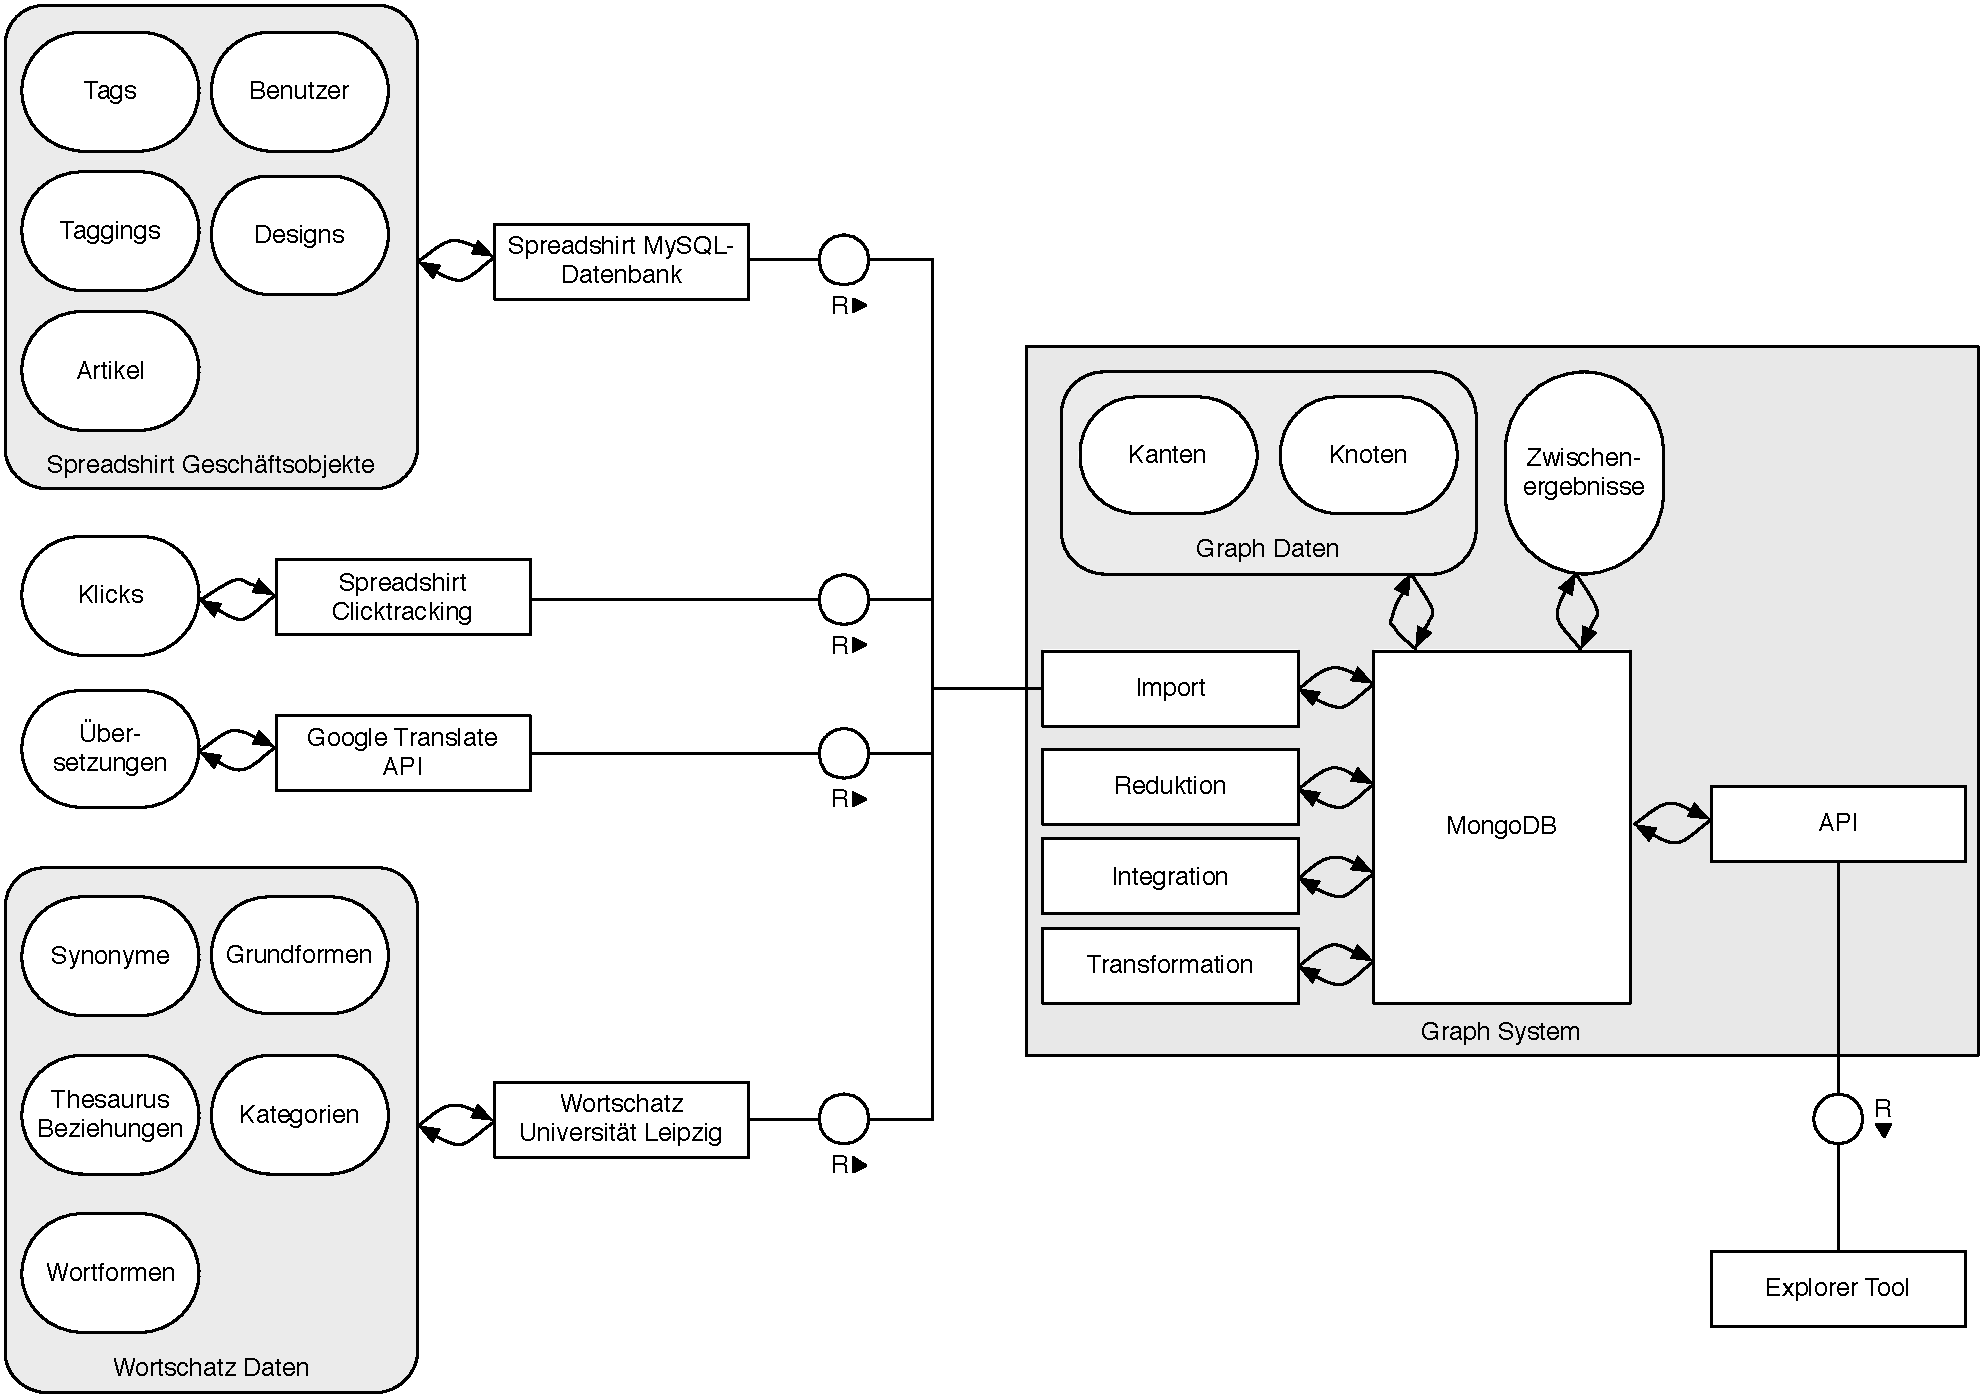
\includegraphics[width=1\textwidth]{architecture}
\caption{Systemarchitektur}
\label{fig:architecture}
\end{figure}

Abbildung \ref{fig:architecture} zeigt die komplette Architektur des implementierten Link Discovery Systems. Darin sind alle genutzten Datenquellen und die Daten, die sie bereit stellen, aufgeführt.

Für jede Datenquelle exisitiert ein Importskript, welches die Rohdaten importiert und in MongoDB speichert. Bei relationalen Datenquellen wie der Spreadshirt MySQL-Datenbank für die Tag-Daten wird pro Tabelle eine Collection und pro Zeile ein Dokument angelegt. Können nicht alle Daten importiert werden, wie beispielsweise bei der Wortschatz-API, kann das Importskript auch aufgrund der bisher im Graph vorhandenen Daten eine Auswahl an Anfragen an die externe Datenquelle erzeugen.

Im nachfolgenden Bereinigungsschritt werden die Daten so gut wie möglich von den in Abschnitt \ref{quality} beschriebenen Defekten befreit. Dazu zählen beispielsweise das Entfernen nicht nutzbarer Zeichen oder unvollständigen Datensätzen.

Der Reduktionsschritt dient zur Verkleinerung der Datenmenge. Dazu gehören beispielsweise Schritte zur Duplikatentfernung oder zur Auswahl relevanter Datensätze. In dieser Arbeit bestand die Haupteinschränkung der Datenmenge darin, nach Möglichkeit nur deutschsprachige Datensätze auszuwählen.

Der Schritt der Transformation überführt die Daten schließlich in eine Graphenform. Dies kann entweder über Kookkurrenz oder über eine andere, für die Art der importierten Daten geeignete, Methode erfolgen.

Das Integrationsskript für jede Datenquelle ist letztendlich für die Integration der Daten in den Zielgraphen verantwortlich. Dabei werden neue Informationen an die Knoten angefügt oder neue Kanten in den Graph integriert. In diesem Schritt passiert die Auflösung von eventuell vorhandenen temporären Bezeichnern in die entsprechenden im Graph vorhandenen eindeutigen Bezeichner.

Für die Abfrage der im Graph gespeicherten Informationen existiert außerdem eine API, welche Informationen zu Knoten und deren Nachbarn per HTTP als JSON-Dokumente zur Verfügung stellt. Diese API kann für die Einbindung der erzeugten Informationen in andere Applikationen genutzt werden. Über Anfrageparameter kann dabei die Gewichtung der einzelnen Kantentypen beeinflusst werden.

Eine Beispielanwendung, die die API des Link Discovery-Systems nutzt, ist der \emph{Tag Explorer}. Dabei handelt es sich um eine Browseranwendung, die die im Graph gespeicherten Beziehungen visualisiert und interaktiv erforschbar macht. Der Benutzer dieser Anwendung kann mit selbst gewählten Gewichtungen der Kanten den Graph durchsuchen. Außerdem werden, wenn vorhanden, über eine Anbindung der Spreadshirt-API zu der Zeichenkette des ausgewählten Knotens gefundene Designs angezeigt. In Abbildung \ref{fig:tag_explorer} ist ein Screenshot dieses Werkzeuges zu sehen.

\begin{figure}
\centering
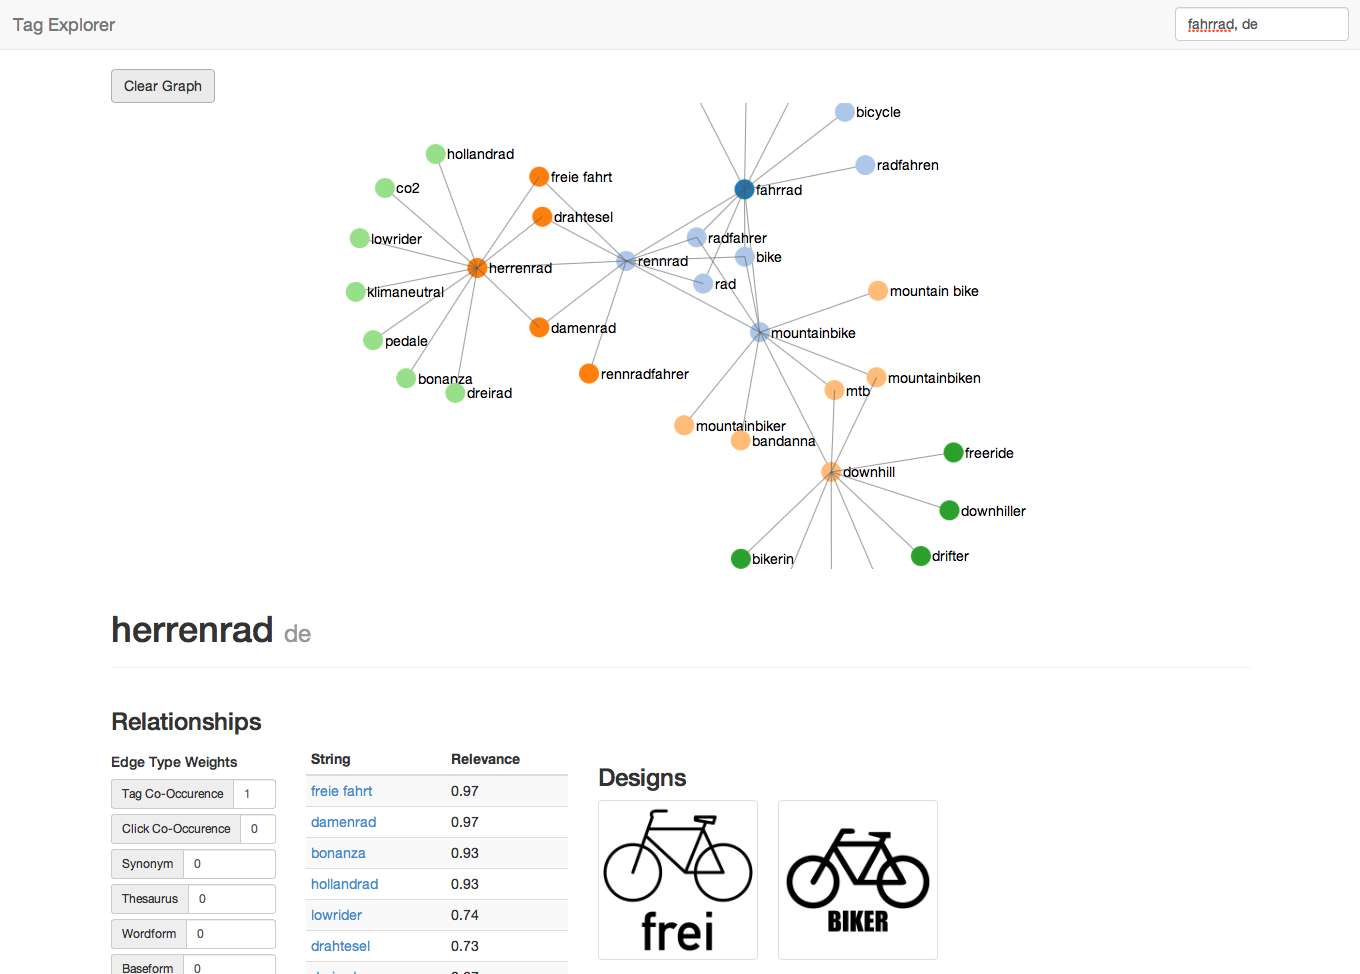
\includegraphics[width=0.9\textwidth]{tag_explorer}
\caption{Tag Explorer}
\label{fig:tag_explorer}
\end{figure}

Nachdem das System zur Link Discovery in diesem Kapitel beschrieben wurde, wird im nächsten Kapitel die praktische Durchführung und die Ergebnisse detailliert beschrieben.
\chapter{Link Discovery}
\label{link_discovery}

Das folgende Kapitel beschäftigt sich mit den im Rahmen dieser Arbeit unternommenen Schritten zur Link Discovery, also dem Finden von Beziehungen zwischen Wörtern und Wortgruppen. Dazu zählen die Generierung eines Ausgangsgraphen aus Tag-Daten, sowie dessen Anreicherung durch die Integration weiterer interner und externer Datenquellen.

\section{Tags}

Den Ausgangspunkt für den in \ref{solution} beschriebenen Lösungsansatz stellen die Daten des Tag-Systems dar. Diese werden in \ref{tag-system} ausführlich beschrieben. Aus diesen Daten wird im ersten Schritt der Zielgraph erstellt, in diesen in allen weiteren Schritten weitere Daten integriert werden. Die in diesem Graph enthaltenen Knoten stellen ebenfalls die Kriterien für die Abfrage der weiteren Datenquellen dar.

Um den Ausgangsgraphen zu berechnen, sind die Schritte des Imports, der Bereinigung, der Reduktion, der Transformation und der Integration notwendig, welche im Folgenden genauer beschrieben werden.

\subsection{Import}

Die Daten liegen im Quellsystem, einer MySQL-Datenbank, in relationaler Form vor. Somit existieren Tabellen für die Tags, Dokumente und Verknüpfungen zwischen ebenjenen. Da der Inhalt der Dokumente nicht relevant für die Link Discovery mittels Kookkurrenz sind, genügt es, die Tabellen der Tags und Verknüpfungen zu importieren.

Die Tags liegen in der Form \((i, s, l)\) vor, wobei \(i\) den eindeutigen Bezeichner des Tags, \(s\) die Zeichenkette und \(l\) die Sprache des Tags repräsentieren.

Die Verknüpfungen sind durch Tupel der Form \((i, t, d_t, d_i)\) repräsentiert, wobei \(i\) der eindeutige Bezeichner der Verknüpfung selbst ist. \(t\) ist der Bezeichner des Tags, \(d_t\) der Typ des Dokuments und \(d_i\) der Bezeichner des Dokumentes. \(d_t\) und \(d_i\) bilden also den zusammengesetzten Schlüssel des getaggten Dokumentes. 
 
\begin{figure}
\centering
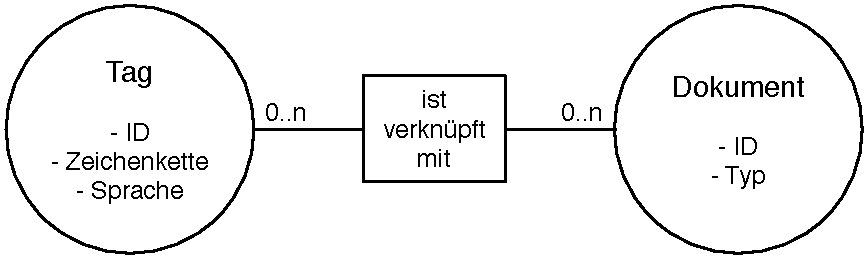
\includegraphics[width=0.6\textwidth]{tag_source_erd}
\caption{Tag-Quelldaten als Entity-Relationship Diagramm}
\label{fig:tag_source_erd}
\end{figure}

\begin{lstlisting}[language=json, label={lst:tag_import_tag}, caption={Beispiele für einen importierten Tag}]
{
    "_id" : ObjectId("51efc20147cae77dfc02e0ac"),
    "tag_id": 12345
    "tag": "segeln",
    "lang": "de"
}
\end{lstlisting}

\begin{lstlisting}[language=json, label={lst:tag_import_link}, caption={Beispiele für eine importierte Verknüpfung eines Tags mit einem Dokument}]
{
    "_id" : ObjectId("51efc20147cae77dfc02e0ac"),
    "object_id": 45678
    "object_type_id": 3,
    "tag_id": 12345
}
\end{lstlisting}

Die importierten Quelldaten sind beispielhaft in den Listings \ref{lst:tag_import_tag} und \ref{lst:tag_import_link} dargestellt. Nach dem Import stehen \num{2072079} Tags und \num{71938905} Verknüpfungen zur Verfügung.

\subsection{Bereinigung}

An den Tag-Daten liegen die in \ref{quality} genannten Defekte in Hinblick auf die Datenqualität vor. Diese sollten in einem Bereinigungsschritt reduziert werden. Hierbei liegt das Hauptaugenmerk auf der Erkennung von Duplikaten und später nicht verwertbaren Zeichenketten. Alle durchgeführten Maßnahmen zur Bereinigung beziehen sich hierbei auf die Eigenschaft \(s\) des Tags, also der Zeichenkette selbst.

In den unbereinigten importierten Daten existieren keine Duplikate in der Art, dass eine Paarung aus Zeichenkette und Sprache immer nur genau einmal in den Daten vorhanden ist. Jedoch enthalten viele der Tags nicht weiter verwertbare Zeichen wie nicht druckbare ASCII Zeichen, Anführungszeichen, Satzzeichen, Sonderzeichen sowie überflüssige Leerzeichen am Anfang und Ende der Zeichenkette. Außerdem existiert in den importierten Daten eine Unterscheidung zwischen Groß- und Kleinschreibung. Diese Unterscheidung bringt im Kontext der Link Discovery keine Vorteile und kann somit entfernt werden.

\begin{table}
\centering
% \arraystretch}{1.3}
\begin{tabular}{lcl}
    \toprule
    Rohdaten & \phantom{abc} & Bereinigte Daten \\
    \midrule
    \textbackslash u0003\textbackslash r\textbackslash nregenbogen && regenbogen \\
    RegenBogen && regenbogen \\
    "Regenbogen" && regenbogen \\
    regenbogen +einhorn && regenbogen einhorn\\
    \phantom{abc} regenbogen && regenbogen \\
    regenbogen && regenbogen \\
    \bottomrule
\end{tabular}
\caption{Beispiele für die Tag-Bereinigung}
\label{tab:tag_cleaning}
\end{table}

Somit besteht der Bereinigungsschritt darin, nicht verwertbare Zeichen zu entfernen und alle Großbuchstaben in Kleinbuchstaben umzuwandeln. Dadurch entstehen Duplikate, welche im darauf folgenden Reduktionsschritt zusammengeführt werden können. In Tabelle \ref{tab:tag_cleaning} sind einige Beispiele für die Bereinigungen aufgeführt. Dabei ist gut zu erkennen, dass durch die Bereinigungen Duplikate erzeugt werden.

\subsection{Reduktion}

Der Reduktionsschritt dient zur Einschränkung der Gesamtdaten auf eine nützliche oder handhabbare Menge. Außerdem kann durch Reduktion auch die Datenqualität verbessert werden.

Im Fall der Tag-Daten liegt das Hauptaugenmerk im Reduktionsschritt auf der Entfernung von Duplikaten, die bei der Bereinigung entstanden sind. Dabei muss gleichzeitig sicher gestellt werden, dass keine Informationen über die Verwendung der Tags verloren gehen. Somit besteht die Duplikatentfernung der Tags im Zusammenführen von Datensätzen mit gleichen Zeichenketten und Sprachen. Dabei werden auch die Verwendungen der Tags zusammengeführt.

Werden die Verknüpfungen zweier Tags mit Dokumenten zusammengeführt, können auch dabei wieder Duplikate entstehen. Diese müssen in diesem Fall entfernt werden, da ein Tag nicht mehrmals mit einem Dokument verknüpft werden kann. Das Zusammenfürhen von Tags ist exemplarisch in Abbildung \ref{fig:tag_reduction} dargestellt.

\begin{figure}
\centering
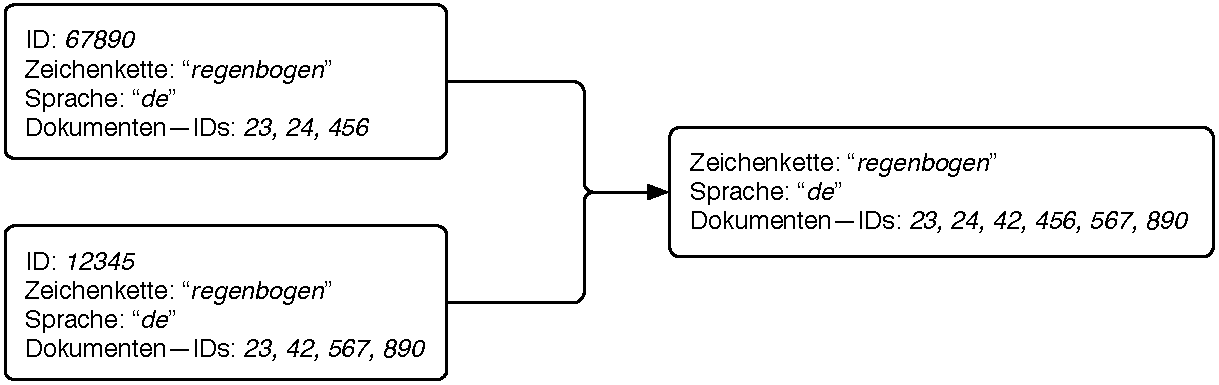
\includegraphics[width=0.7\textwidth]{tag_reduction}
\caption{Beispiel für das Zusammenführen der bereinigten Tags}
\label{fig:tag_reduction}
\end{figure}

Dabei findet ebenfalls eine Denormalisierung der Daten statt, da alle Dokumente, für die ein Tag vergeben werden, direkt mit in das Tag-Dokument gespeichert werden. Dies ist beispielhaft in Listing \ref{lst:tag_denormalization} abgebildet. Dabei enthält das Attribut \emph{links} alle Verknüpfungen des Tags mit Dokumenten.

\begin{lstlisting}[language=json, label={lst:tag_denormalization}, caption={Denormalisierte Tag-Daten}]
{
    "_id" : ObjectId("51efc20147cae77dfc02e0ac"),
    "string": "segeln"
    "language": "de",
    "links": [
        {
            object_id: 45678, 
            object_type_id: 3
        },
        {
            object_id: 98764, 
            object_type_id: 4
        },
        ...
    ]
}
\end{lstlisting}

Eine weitere im Rahmen dieser Arbeit unternommene Maßnahme zur Datenreduktion bestand darin, sich auf die Menge der Tags zu beschränken, deren Attribut \(l\) den Wert \emph{de} besitzt. Praktisch handelt es sich dabei um alle Tags, die als deutsch gekennzeichnet in der Datenbank gespeichert sind. Diese Einschränkung wurde vorgenommen, um die zu verarbeitende Datenmenge überschaubar zu halten. Außerdem wird dadurch der nationale Kontext, in dem die Begriffe verwendet wurden, weitestgehend beibehalten.

Ein letzter Reduktionsschritt besteht in der Entfernung der Tags, deren Zeichenketten eine Länge von \num{1} besitzen, da in der deutschen Sprache keine einbuchstabigen Wörter existieren.

Nach der beschriebenen Reduktion befinden sich noch \num{314351} Tags und \num{23255714} Verknüpfungen in der Datenbank. Dies entspricht einer Reduktion von ca. \num{68} Prozent gegenüber der importierten Menge von Objekten.

\subsection{Transformation}

Der Transformationsschritt beschreibt die Überführung der Daten in die Form, die für das Ergebnis benötigt wird. Im Falle der Tag-Daten bedeutet dies eine Umformung in die Form des Kokkurrenzgraphen, also die Erzeugung von Knoten- und Kantenobjekten. Die Umsetzung dieser Transformation mittels des Programmiermodells MapReduce wurde in \ref{mapreduce_cooccurence} genauer beschrieben.

Je Tag wird ein Datenbankdokument erzeugt, dass den Knoten repräsentiert. Dieses besitzt als Attribute zum einen die Zeichenkette und die Sprache des Tags, aus dem es erzeugt wurde. Zum anderen wird ein Unterdokument hinzugefügt, welches weitere Eigenschaften des Ausgangstags beschreibt. Die umfasst die Anzahl der Verwendungen und die eindeutigen Bezeichner der Dokumente, also Artikel oder Designs, die mit dem Tag getaggt wurden. Außerdem wird im Transformationsschritt für jeden Knoten ein global eindeutiger Bezeichner erzeugt, um das spätere Referenzieren der Knoten einfacher zu machen. Zeichenkette und Sprache des Knotens stellen einen zusammengesetzten Schlüssel dar und sind in der Knotenmenge eindeutig. Listing \ref{lst:tag_transform_node} zeigt ein Beispiel für ein in der Datenbank abgelegtes Knotendokument.

\begin{lstlisting}[language=json, label={lst:tag_transform_node}, caption={Tag-Knoten als JSON-Dokument}]
{
    "_id" : ObjectId("51efc20147cae77dfc02e0ac"),
    "language" : "de",
    "string" : "mama",
    "tagProperties" : {
        "occurenceCount" : 3,
        "articleCount" : 2,
        "designCount" : 1,
        "articleIDs" : [
            24231101,
            24231105
        ],
        "designIDs" : [
            15514592
        ]
    }
}
\end{lstlisting}

Die Erzeugung der Kanten erfolgt wie in Abschnitt \ref{mapreduce_cooccurence} beschrieben. Dabei werden für jedes gemeinsame Auftreten von zwei Tags zwei Datenbankdokumente erzeugt. Dieses beschreiben gerichtete Kanten zwischen den Tags, die ein gemeinsames Auftreten der Tags repräsentieren. Neben Quell- und Zielknoten enthält eine Kante den Kantentyp sowie weitere Informationen über die Art der Verbindung. Im Fall von Kookkurrenzkanten ist dies zum einen die absolute Anzahl gemeinsamer Vorkommen der Tags, zum anderen die in \ref{measures} beschriebenen Kookkurrenzmaße. Der Kantentyp ist aus der Berechnung folgend der Typ der Tag-Kookkurrenz. Ein Beispiel JSON-Dokument für eine Kante ist in Listing \ref{lst:tag_transform_edge} zu sehen.

\begin{lstlisting}[language=json, label={lst:tag_transform_edge}, caption={Tag-Kante als JSON-Dokument}]
{
    "_id" : ObjectId("51efd6f61177ff360605bd99"),
    "source" : ObjectId("51efc1af47cae77dfc00c3f8"),
    "target" : ObjectId("51efc1e047cae77dfc02087c"),
    "type" : "tag-co-occurence",
    "occurences" : 1,
    "dice" : 0.0001317089232795522,
    "jaccard" : 0.00006585879873551106,
    "cosine" : 0.008115343414514944
}
\end{lstlisting}

\subsection{Integration}

Da der aus den Tag-Daten generierte Kookkurrenzgraph die Ausgangsbasis für alle weiteren Operationen darstellt, muss im Sinne der Integration nichts getan werden. Die transformierten Daten müssen lediglich in die Zieldatenbank kopiert werden.

Durch die Schritte, die zur Link Discovery aus den Tag-Daten verwendet wurden, wurden insgesamt \num{314351} Knoten und \num{21834868} Kanten erzeugt, welche nun durch weitere Schritte angereichert werden sollen.

\section{Clicktracking}
\label{clicktracking}

Spreadshirt betreibt ein Clicktracking-System, welches die Klicks der Benutzer auf Artikel und Designs auf Suchergebnisseiten aufzeichnet. Dabei ist unerheblich, ob der Benutzer bei Spreadshirt registriert und angemeldet ist. Dieses System sammelt Daten von beiden Spreadshirt-Plattformen (siehe \ref{platforms}). In Abbildung \ref{fig:search_result} ist beispielhaft eine Suchergebnisseite der Spreadshirt-Plattform abgebildet, welches die gefundenen Designs für eine Suchanfrage auflistet.

\begin{figure}
\centering
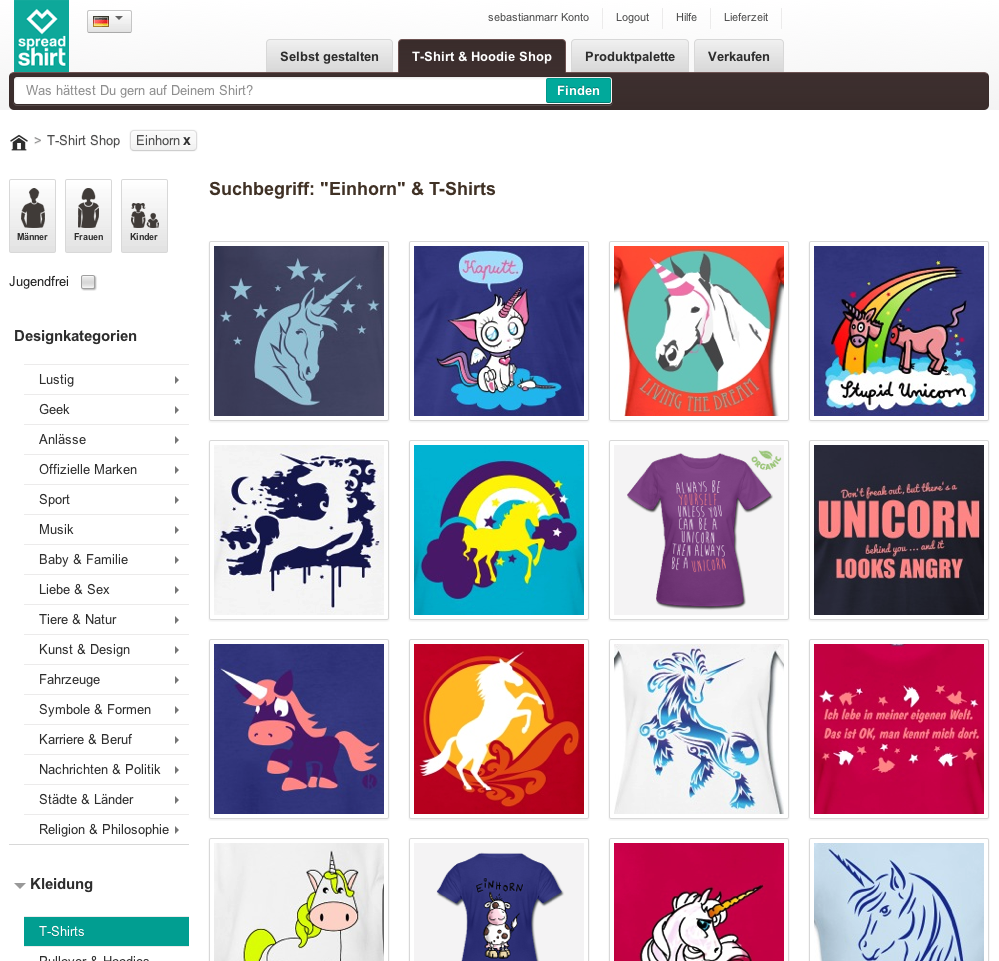
\includegraphics[width=\textwidth]{search_result}
\caption{Suchergebnisseite}
\label{fig:search_result}
\end{figure}

Die von diesem System erzeugten Daten können für die Link Discovery von großer Bedeutung sein, da sie eine andere Perspektive auf die Begriffe im Graphen liefern. Die Tags liefern die Sicht der Partner, also der Personen, die Inhalte hochladen und verkaufen möchten. Die Klicks beschreiben die Sicht der Käufer, also der Personen, die nach Inhalten suchen. Durch die Auswertung der Clicktracking-Daten ergibt sich also die Möglichkeit, eine Form der Validierung der durch Partner vergebenen Metadaten zu erhalten. Die Annahme hierbei ist, dass Käufer nur auf Suchergebnisse klicken, die eine inhaltliche Relevanz zum eingegebenen Suchbegriff besitzen und somit ihren Erwartungen bezüglich des Suchbegriffes gerecht werden.

Wie bereits für die Tag-Daten, werden im Folgenden auch für das Clicktracking die Schritte Import, Bereinigung, Reduktion, Transformation und Integration näher erläutert. Der Ansatz zur Erzeugung der Verbindungen ist ebenfalls kookkurrenzbasiert.

\subsection{Import}
\label{click_import}

Das Clicktracking-System erzeugt Dateien im JSON-Format, die zu jedem Klick auf einer Ergebnisseite die wesentlichen Informationen enthalten. Dabei ist pro Klick ein JSON-Dokument in den Dateien abgespeichert. Ein Beispiel für ein solches Dokument ist in Listing \ref{lst:click_raw} dargestellt.

\begin{lstlisting}[language=json, label={lst:click_raw}, caption={Clicktracking - Rohdokument als JSON}]
{
    "date": "01.07.2013 00:09:31_633",
    "path": "/track/eu/205909/1E3B6E3E-4496-C51A14A8FA25/2.10.4/list",
    "params": {
        "locale": "[de_DE]",
        "search-query": "[biene]",
        "cl": "[a18869874, p25446183, i49]"
    }
}
\end{lstlisting}

Ein Clicktracking-Dokument enthält dabei die Attribute \emph{Datum}, \emph{Pfad}, \emph{Gebietsschema}, \emph{Suchbegriff} und die Daten des eigentlichen Klicks, also den geklickten \emph{Artikel}, das geklickte \emph{Produkt} und den \emph{Index}, also die Position des geklickten Inhaltes auf der Suchergebnisseite. Die Unterscheidung zwischen Produkt und Artikel ist dabei im Domänenmodell von Spreadshirt begründet (siehe auch \ref{spreadshirt} und für die Link Discovery nicht von Interesse. Es genügt, den geklickten Artikel im Weiteren näher zu betrachten.

Auffällig ist, dass die Möglichkeiten des JSON-Formates bei der Speicherung der Klickdaten nicht vollständig ausgenutzt wurden. So sind die Werte, die das geklickte Dokument beschreiben, als Zeichenkette abgelegt und zusätzlich die eindeutigen Bezeichner mit einem Buchstaben versehen, der ihren Typ angibt. Des weiteren enthalten  das Gebietsschema und der Suchbegriff zusätzliche eckige Klammern. Diese Defekte sollten im Bereinigungsschritt beseitigt werden, um ein nutzbareres Datenformat zu erhalten.

Da das Clicktracking-System zum Zeitpunkt des Imports erst 3 Monate Daten aufzeichnete, standen \num{2249942} solcher Klickdokumente zur Verfügung.

\subsection{Bereinigung}

Im Bereinigungsschritt müssen zunächst die genannten Defekte der Klickdaten beseitigt werden. Dazu gehört die Entfernung der eckigen Klammern in Suchbegriff und Gebietsschema und die Extraktion des eindeutigen Bezeichners des geklickten Artikels. Aus dem Gebietsschema ist nur die Sprache von Interesse. Außerdem wurden für den Suchbegriff die gleichen Bereinigungsoperationen wie für die Tag-Daten vorgenommen, also die Entfernung von überflüssigen Leerzeichen, Groß-/Kleinschreibung, nicht druckbarer Sonderzeichen und Satzzeichen.

Im Bereinigunsschritt werden so auch einfacher verarbeitbare Dokumente erzeugt, da die Möglichkeiten des JSON-Formates besser ausgenutzt werden. Listing \ref{lst:tag_cleanup} zeigt das Ergebnis der Bereinigung des in \ref{click_import} gezeigten Beispieldokumentes.

\begin{lstlisting}[language=json, label={lst:tag_cleanup}, caption={Bereinigtes Clicktracking-Dokument}]
{
    "_id": ObjectId("51e7b1e0417498f9c6868939"),
    "query" : "biene",
    "date" : "2013-07-01T00:09:31.633Z",
    "articleId" : 18869874,
    "index" : 57,
    "language" : "de"
}
\end{lstlisting}

\subsection{Reduktion}

Die Reduktion der Clicktracking-Daten besteht zum einen aus einer Duplikatentfernung, zum anderen aus der Einschränkung der Sprache.

Im Sinne der Kookkurrenz ist es nicht von Bedeutung, wenn Paare aus Suchbegriffen und geklickten Artikeln mehrfach auftauchen, da hierfür nur das gemeinsame Auftreten unterschiedlicher Suchbegriffe betrachtet wird. Somit besteht die Duplikatentfernung lediglich darin, aus mehrfach vorkommenden Artikel-/Klickpaaren genau eines auszuwählen.

Außerdem erfolgte, wie schon bei den Tag-Daten, eine Einschränkung auf Klicks, die als \emph{deutsch} gekennzeichnet sind.

Nach dem Reduktionsschritt verblieben zur Transformation noch \num{411341} Klicks.

\subsection{Transformation}

Im Transformationsschritt wird für die Clicktracking-Daten ein Kookkurrenzgraph berechnet. Die Kookkurrenz bestimmt sich hierbei daraus, welche Suchbegriffe zum Klick auf einen Artikel geführt haben. Wird ein Artikel zu mehreren Suchbegriffen geklickt, liegt die Vermutung nah, dass zwischen den Suchbegriffen ein irgendwie gearteter Zusammenhang besteht.

Ziel der Transformation ist somit die Erzeugung von Knoten und Kanten. Die Knoten besitzen dabei zusätzliche Eigenschaften, die die Eigenschaften des durch den Knoten repräsentierten Begriffes im Kontext des Clicktrackings widerspiegeln. Konkret sind dies die Artikel, die zu dem Begriff als Suchbegriff geklickt wurden. Listing \ref{lst:click_node} zeigt beispielhaft ein erzeugtes Knotendokument.

\begin{lstlisting}[language=json, label={lst:click_node}, caption={Knotendokument mit Clicktracking-Eigenschaften}]
{
    "_id": ObjectId("51e7f1e04146498f9c6868945"),
    "string": "biene",
    "language": "de",
    "clickProperties": [
        { "articleId": 4512 },
        { "articleId": 4794 },
        ...
    ]
}
\end{lstlisting}

Die Kanten besitzen die gleiche Form wie die Kookkurrenzkanten, die bei der Integration der Tag-Daten erzeugt wurden. Ein Beispiel für ein solches Kantendokument ist in Listing \ref{lst:click_edge} dargestellt.

\begin{lstlisting}[language=json, label={lst:click_edge}, caption={Clicktracking-Kookkurrenzkante}]
{
    "_id": ObjectId("51e91aff3b6a20bfd68c468a")
    "source" : ObjectId("51e91af93b6a20bfd68b0bed"),
    "target" : ObjectId("51e91aff3b6a20bfd68c463e"),
    "type": "tag-co-occurence",
    "occs" : 1,
    "dice" : 0.003883495145631068,
    "jaccard" : 0.0019455252918287938,
    "cosine" : 0.04410810913912309
}
\end{lstlisting}

Die Durchführung des Transformationsschrittes erfolgte ebenfalls mittels MapReduce (siehe \ref{mapreduce_cooccurence}). Dadurch wurden \num{92727} Knoten und \num{310860} Kanten erzeugt.

\subsection{Integration}
\label{click_integration}

Die Integration der erzeugten Daten stellt eine Vereinigung des vorhandenen Zielgraphen mit dem im Transformationsschritt erzeugten Kookkurrenzgraphen dar.

Dabei wird die Knotenmenge derart vereinigt, dass die Knotenmenge des Zielgraphen die Eigenschaft behält, dass Paare aus Sprache und Zeichenkette eindeutig sind. Somit werden bei bereits vorhandenen Knoten die zusätzlichen Informationen bezüglich das Clicktrackings als Attribute hinzugefügt. Existiert eine Kombination aus Sprache und Zeichenkette noch nicht im Zielgraph, so wird der entsprechende Knoten kopiert.

Da die erzeugten Kanten einen noch nicht im Graph vorhandenen Typ besitzen, müssen keine Kanten zusammengeführt werden. Jedoch werden die Bezeichner der Ziel- und Quellquoten entsprechend angepasst, wenn bei der Integration der Knoten eine Zusammenführung stattgefunden hat.

Durch dieses Vorgehen konnten der Knotenmenge \num{78237} Knoten, und somit auch neue Begriffe hinzugefügt werden. Die Kantenmenge wurde, wie bereits erläutert, um \num{310860} Kanten erweitert.

\section{Google Translate}

Google bietet im Rahmen seines \emph{Translate}-Services \cite{gt2013} eine kostenpfichtige API für Spracherkennung an. Diese ermöglicht es, die Sprache beliebiger Zeichenketten automatisch erkennen zu lassen. Google stellt hierzu eine API zur Verfügung.

Diese Schnittstelle liefert Ergebnisse der Form \((l, c)\), wobei \(l\) die für die Zeichenkette erkannte Sprache und \(c\) einen Konfidenzwert für die Spracherkennung repräsentiert. Der Konfidenzwert liegt dabei im Intervall zwischen \num{0} und \num{1} und stellt die Verlässlichkeit der Spracherkennung dar.

Die Integration der Spracherkennungs-Daten in den Graphen gestaltet sich einfach. Dazu werden die durch die bereits vorhandenen Knoten repräsentierten Zeichenketten extrahiert und als Eingabedaten für die Spracherkennungs-API verwendet. Die Ergebnisse werden abgespeichert, um weitere kostenpflichtige Abfragen zu vermeiden.

Eine Bereinigung der Ergebnisse ist nicht erforderlich. Somit müssen die Ergebnisse lediglich in den Ausgangsgraphen integriert werden. Die Spracherkennung an sich bringt keine Ähnlichkeitsbeziehungen mit sich, sondern verbessert gegebenenfalls nur die Knotenauswahl für spätere Operationen.

In der Konsequenz genügt es also, die für die Abfrage verwendeten Knoten mit den Ergebnissen der Spracherkennung zu annotieren. Somit kann dann bei späteren Analysen anhand des Konfidenzwertes abgewogen werden, ob die erkannte Sprache oder die eventuell schon am Knoten vorhandene Sprache verwendet werden soll. Ein resultierender Knoten ist in Listing \ref{lst:google_node} abgebildet.

\begin{lstlisting}[language=json, label={lst:google_node}, caption={Knoten mit Spracherkennungsdaten}]
{
    "_id" : ObjectId("51efc1dc47cae77dfc01ea43"),
    "language" : "de",
    "string" : "grey head",
    "languageDetection" : {
        "language" : "en",
        "confidence" : 0.7105263000000001
    }
}
\end{lstlisting}

\section{Zerlegung von Wortgruppen}

Die Zerlegung von Tags, die aus mehr als einem Wort bestehen, stellt zwar keine Integration anderer Datenquellen dar, kann aber trotzdem zum Auffinden neuer Verknüpfungen nützlich sein. Außerdem kann es für weitere Integrationsschritte von Nutzen sein, möglichst viele Einzelwörter im Datenbestand zu haben (siehe auch \ref{wortschatz}).

Zum Zeitpunkt des Importes befanden sich \num{147364} Tags in der Datenbank, die aus mehreren Wörtern bestehen. Dies entspricht \num{47} Prozent aller bereinigten deutschen Tags. Dieser Umstand legt die Vermutung nahe, dass in diesen zusammengesetzten Tags auch Wörter enthalten sind, die nicht als Einzelwörter existieren.

Werden diese Tags in ihre Einzelwörter zerlegt, entstehen einerseits unter Umständen neue Knoten, andererseits können in diesem Schritt Kanten vom Typ \emph{Zerlegung} beziehungsweise \emph{Zusammensetzung} eingefügt werden. Somit sind nach dem Zerlegungsschritt weitere Informationen über den Kontext, in dem Wörter verwendet werden, verfügbar. Abbildung \ref{fig:decomposition} zeigt beispielhaft das Ergebnis einer solchen Zerlegung.

Durch die Anwendung des Zerlegungsschrittes auf die vorhandenen Tag-Daten wurden insgesamt \num{38349} Knoten und \num{1238900} Kanten erzeugt, die für spätere Analyseschritte genutzt werden können.

\begin{figure}
\centering
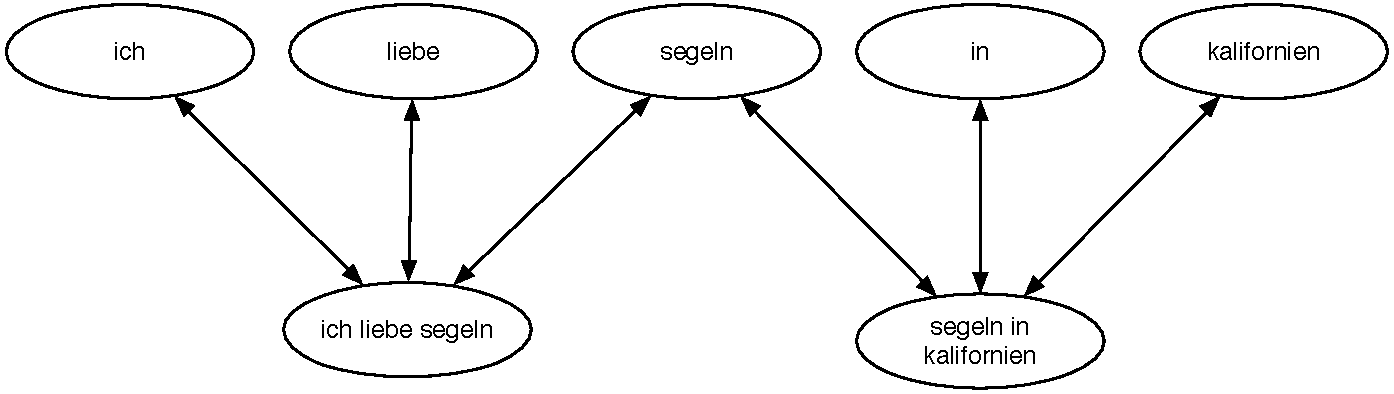
\includegraphics[width=\textwidth]{decomposition}
\caption{Beispielhafter Graphausschnitt nach der Zerlegung}
\label{fig:decomposition}
\end{figure}

\section{Wortschatz der Universität Leipzig}
\label{wortschatz}

Die Universität Leipzig betreibt ein Wortschatz-Projekt \cite{ws2013}. Im Rahmen dieses Projektes wird durch die Analyse von großen Textmengen eine Datenbank deutscher Wörter, deren Bedeutungen, grammatikalische Eigenschaften, Häufigkeiten und Kookkurrenzen in Texten und Beziehungen zu anderen Wörtern aufgebaut. Somit stellt dieses Projekt eine sehr gute Möglichkeit dar, weitere Beziehungen zwischen den schon im Graph vorhandenen Knoten herzustellen. Neben den Daten, die im Spreadshirt-Kontext entstehen, können somit auch allgemeine linguistische Daten hinzugefügt und für spätere Analysen genutzt werden.

Neben dem Webportal stellt dieses Projekt eine API bereit, über die die Daten des Wortschatz programmatisch abgefragt werden können. Diese API wurde mittels einer Ruby-Bibliothek \cite{wlapi2013} im Rahmen dieser Arbeit für einen weiteren Integrationsschritt zur Link Discovery genutzt.

Für jedes Wort als Eingabeparameter stellt die Wortschatz-API die folgenden Informationen bereit:

\begin{itemize}
    \item Grundform des Wortes
    \item Wortformen
    \item Kookkurrenzen in den analysierten Texten
    \item Kategorien, in die das Wort eingeordnet werden kann
    \item Synonyme
    \item Thesaurus-Beziehungen
    \item Häufigkeit des Auftretens
    \item Sätze, die das Wort enthalten
\end{itemize}

Für die Link Discovery wurden die Informationen \emph{Grundform}, \emph{Wortformen}, \emph{Kategorien}, \emph{Synonyme} und \emph{Thesaurus-Beziehungen} genutzt.

Wie bereits für die anderen Datenquellen, werden im Folgenden auch für den Wortschatz die Schritte des Imports, der Bereinigung, der Reduktion, der Transformation und der Integration beschrieben.

\subsection{Import}

Da für die Anfrage an die Wortschatz-API nur Einzelwörter und keine Wortgruppen genutzt werden können, muss eine Auswahl der anzufragenden Daten getroffen werden. Im Rahmen dieser Arbeit wurden alle Einzelwörter, die zum Zeitpunkt des Importes der Wortschatz-API zur Verfügung standen, ausgewählt. Dabei handelt es sich um \num{197614} einzelne Wörter. Da die Daten in der Datenbank zu diesem Zeitpunkt keine Groß- und Kleinschreibung enthielten, die Wortschatz-API diese jedoch berücksichtigt, wurde jedes Wort jeweils groß und klein geschrieben angefragt. Somit wurde die doppelte Menge an Datensätzen, \num{395228} Dokumente, erzeugt.

Die Ergebnisse wurden mittels eines Ruby-Skriptes in MongoDB importiert. Dabei wurde je angefragtem Wort ein Dokument erzeugt, dass die Wortschatz-Informationen enthält. Eines dieser Dokumente ist beispielhaft in Listing \ref{lst:wortschatz_import} dargestellt. Das Feld \emph{baseform} enthält dabei die Grundform des Wortes mit der Wortart und \emph{domain} die Kategorien des Wortes.

\begin{lstlisting}[language=json, label={lst:wortschatz_import}, caption={Wortschatz-Dokument nach dem Import}]
{
    "_id" : ObjectId("51f7aa06eba16044e900015a"),
    "string" : "Kopf",
    "baseform" : [ 
        "Kopf", 
        "N"
    ],
    "domain" : [ 
        "Medizin", 
        "Anatomie", 
        "Literarische/Motive/Stoffe/Gestalten", 
        "Körperteile"
    ],
    "synonyms" : [  
        "Chef", 
        "Figur", 
        "Gestalt", 
        "Haupt", 
        "Jemand", 
        "Individuum", 
        "Figur"
    ],
    "thesaurus" : [ 
        "Titel", 
        "Hand", 
        "Kopf", 
        "Mensch", 
        "Gesicht", 
        "Spitze", 
        "Arm", 
        "Gestalt"
    ],
    "wordforms" : [ 
        "Kopf", 
        "Köpfe", 
        "Köpfen", 
        "Kopfes", 
        "Kopfs"
    ]
}
\end{lstlisting}

Hierbei ist zu beachten, dass nicht alle Attribute bei allen Wörtern vorhanden sind. Dies hängt davon ab, ob der Wortschatz die Informationen zur Verfügung stellen kann. Somit ist es auch möglich, dass Dokumente erzeugt werden, die keine zusätzlichen Informationen enthalten.

\subsection{Bereinigung}

Zur Bereinigung der importierten Wortschatz-Daten muss in einem ersten Schritt die Groß- und Kleinschreibung entfernt werden, da diese an erster Stelle nur für die Anfragen an die API wieder in den Datenbestand eingeführt wurde.

Weiterhin werden die Kategorien ``Vorname'' und ``Nachname'' entfernt, da diese an über \num{25000} Wörter vergeben sind und somit für die Verwendung zur Link Discovery ungeeignet sind und zu viele irrelevante Kanten erzeugen würden.

Ein letzer Bereinigungsschritt besteht in der Veränderungen des Formates der Grundform des Wortes. Die Wortschatz-API liefert lediglich ein Array, in dem das erste Element die Grundform und das zweite Element die Wortart ist. Zur Bereinigung wird diese Eigenschaft in ein geeignetes JSON-Format überführt, welches in Listing \ref{lst:word_baseform} dargestellt ist.

\begin{lstlisting}[language=json, label={lst:word_baseform}, caption={Grundform eines Wortes}]
{
    _id: ...,
    string: "Kopfs",
    baseform: {
        word: "Kopf",
        type: "N"
    }
}
\end{lstlisting}

\subsection{Reduktion}

Der Reduktionsschritt besteht in der Zusammenführung von Dokumenten mit gleichen Wörtern, welche im Bereinigungsschritt entstanden sind. Wie schon bei der Reduktion der Tag-Daten, muss auch hierbei das Entstehen neuer Duplikate vermieden werden. Dies bedeutet, dass die gefundenen Wortbeziehungen ebenfalls zusammengeführt werden, wobei jedes verbundene Wort nur einmal enthalten sein darf. Die Reduktion ist beispielhaft in Abbildung \ref{fig:wortschatz_reduction} dargestellt. Dabei ist zu beachten, dass bei der Zusammenführung mehrere Grundformen entstehen können, wodurch dieses Attribut in ein Array umgewandelt wird.

\begin{figure}
\centering
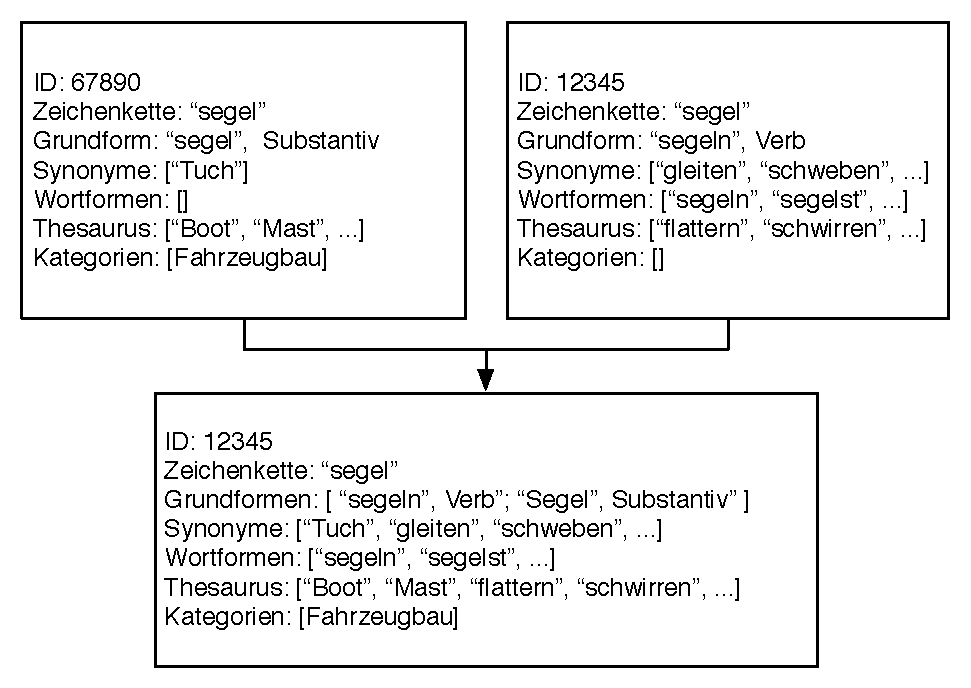
\includegraphics[width=0.8\textwidth]{wortschatz_reduction}
\caption{Reduktion der Wortschatz-Daten}
\label{fig:wortschatz_reduction}
\end{figure}

Durch die Reduktion wird die Anzahl der Dokumente auf die Hälfte reduziert und beträgt danach \num{197614}.

\subsection{Transformation}

Die Transformation der Wortschatz-Daten besteht, wie bereits bei den anderen Datenquellen, in einer Überführung in eine Graph-Datenstruktur. 

Die Knoten sind dabei alle Wörter, die durch die Benutzung der Wortschatz-API bekannt sind. Dazu zählen einerseits sowohl die angefragten Wörter, als auch die verbundenen Wörter, die die API liefert.

Die Kanten werden dabei jeweils für die Attribute \emph{Synonyme}, \emph{Thesaurus}, \emph{Grundform} und \emph{Wortformen} erzeugt und besitzen die entsprechenden Kantentypen. Sie besitzen keine weiteren Attribute, da über diese Beziehungen keine weiteren Informationen verfügbar sind.
\begin{figure}
\centering
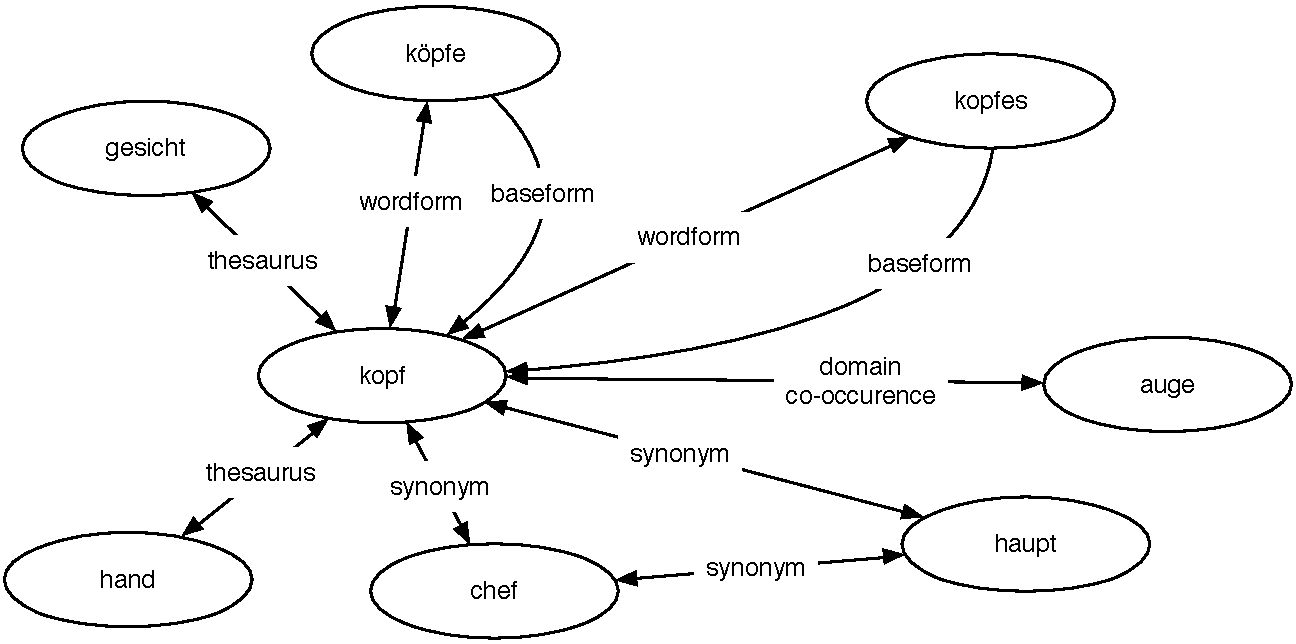
\includegraphics[width=\textwidth]{wortschatz_transformation}
\caption{Wortschatz-Daten in Graphenform}
\label{fig:wortschatz_transformation}
\end{figure}

Einen Sonderfall stellen dabei die Kategorien der Wörter dar. Diese können in der vorliegenden Form nicht zur Link Discovery genutzt werden. Daher werden diese Daten mittels der Ermittlung von Kookkurrenzen umgeformt. Von Interesse ist dabei wie oft Paare von Wörtern 
in gemeinsame Kategorien eingeordnet sind. 

Somit werden bei der Transformation mittels MapReduce (siehe \ref{mapreduce_cooccurence}) Kanten mit den Kookkurrenzmaßen Dice, Jaccard und Kosinus erzeugt.

Zusammenfassend werden bei der Transformation demnach Kanten der Typen \emph{Synonym}, \emph{Thesaurus}, \emph{Wortform}, \emph{Grundform} und \emph{Kategorie-Kookkurrenz} erzeugt. Abbildung \ref{fig:wortschatz_transformation} zeigt beispielhaft einen Ausschnitt des resultierenden Graphen. Dabei fällt auf, dass mit Ausnahme der Grundform-Kanten jede Kante in beide Richtungen existiert. Dies ist der Art der Beziehungen geschuldet, da diese in beide Richtungen gültig sind.

\subsection{Integration}

Zur Integration wird der im Transformationsschritt erzeugte Graph mit dem Zielgraphen vereinigt. Diese Vereinigung wird analog zur Integration der Clicktracking-Daten in Abschnitt \ref{click_integration} durchgeführt.

Insgesamt wurden dadurch \num{145023} neue Knoten und \num{50227965} neue Kanten erzeugt.  Dabei entfallen \num{48399466} Kanten auf Kookkurrenz von Kategorien, \num{550270} Kanten auf Wortformen, \num{149381} Kanten auf Grundformen, \num{279118} Kanten auf Synonyme und \num{849730} Kanten auf Thesaurus-Beziehungen.

Nachdem alle vorgenommen Schritte zur Link Discovery beschrieben wurden, beschäftigt sich der nächste Abschnitt mit einer Zusammenfassung der Ergebnisse.

\section{Ergebnisse}

Im folgenden Abschnitt werden die quantitativen Ergebnisse der Link Discovery zusammenfassend dargestellt und diskutiert.

\begin{table}
\centering
\begin{tabular}{lrcr}
    \toprule
    Schritt & Knoten & \phantom{abc} & Kanten \\
    \midrule
    Tags & \num{314351} && \num{21834868} \\
    Clicktracking & \num{78237} && \num{310860} \\
    Zerlegung & \num{38349} && \num{1238900} \\
    Wortschatz & \num{145023} && \num{50227965} \\
    \midrule
    Gesamt & \num{575960} && \num{73612593} \\
    \bottomrule
\end{tabular}
\caption{Quantitative Ergebnisse der Link Discovery-Schritte}
\label{tab:discovery_amounts}
\end{table}

Tabelle \ref{tab:discovery_amounts} führt für jeden Schritt die hinzugefügten Knoten und Kanten sowie die nach Durchführung der Link Discovery insgesamt im Graphen enthaltene Datenmenge auf. Dabei zeigt sich, dass die Integration der Wortschatzdaten mit Abstand die meisten neuen Kanten in den Graphen eingefügt hat. 

Bei der Verwendung der Clicktracking-Daten wurden im Verhältnis wenig neue Knoten und Kanten erzeugt. Dies ist im Wesentlichen auf den zum Zeitpunkt des Importes noch geringen Datenbestand zurückzuführen. Daher sollte dieser Schritt zukünftig wiederholt werden, da mit der längeren Laufzeit des Clicktracking-Systems auch ein größeres Potential für neue Verknüpfungen vorhanden ist.

Die Integration von Google Translate brachte weder neue Knoten noch Kanten, da in diesem Schritt bewusst nur neue Attribute zu vorhandenen Knoten hinzugefügt wurden.

Neben der absoluten Anzahl der Knoten und Kanten sind bei einer Betrachtung der quantitativen Ergebnisse auch die Anzahl der Kanten, die von einem Knoten ausgehen, von Interesse. Tabelle \ref{tab:discovery_edges_per_node} zeigt die Entwicklung der Kantenanzahl pro Knoten nach jedem Link Discovery-Schritt. Dabei sind Minimum, das untere, mittlere (Median) und obere Quartil, das Maximum und der Durchschnitt dargestellt, um die Verteilung der Kantenanzahl zu verdeutlichen.

\begin{table}
\centering
\begin{tabular}{lrrrrrr}
    \toprule
    Schritt & \(min\) & \(Q_{0.25}\) & \(Q_{0.5}\) & \(Q_{0.75}\) & \(max\) & \(avg\) \\
    \midrule
    Tags & \num{0} & \num{8} & \num{15} & \num{26} & \num{35170} & \num{69,64} \\
    Clicktracking & \num{0} & \num{3} & \num{10} & \num{23} & \num{35170} & \num{56,41} \\
    Zerlegung & \num{0} & \num{4} & \num{11} & \num{24} & \num{37940} & \num{54,26} \\
    Wortschatz & \num{0} & \num{2} & \num{8} & \num{23} & \num{38380} & \num{127,8} \\
    \bottomrule
\end{tabular}
\caption{Entwicklung der Anzahl der Kanten von einem Knoten ausgehend}
\label{tab:discovery_edges_per_node}
\end{table}

Auffällig ist hierbei, dass die Integration von Clicktracking- und Wortschatz-Daten zu einer Herabsenkung des Medians führten. Dies bedeutet, dass verhältnismäßig nach Durchführung dieser Schritte weniger vielverbundene Knoten im Datenbestand existierten als davor. Jedoch deutet die Entwicklung des Durchschnittes nach der Integration der Wortschatz-Daten darauf hin, dass die Knotenanzahl vielverbundener Knoten nach diesem Schritt deutlich größer geworden ist.

Das Absinken des Durchschnittes nach Integration der Clicktracking-Daten kann dabei in der geringen Menge der Daten begründet werden. Durch die geringe Anzahl von Kookkurrenzen konnten vielverbundene Knoten keinen relevanten Zugewinn an Verbindungen verzeichnen, während für wenig verbundene Knoten verhältnismäßig mehr neue Verbindungen hinzukamen.

Generall lässt sich festhalten, dass die Anzahl vielverbundener Knoten gemessen an der Gesamtanzahl relativ klein ist. Die Auswirkungen dessen hängen jedoch stark von der Anwendung der Daten ab und sind im Rahmen dieser Arbeit nicht beurteilbar.

Nach der quantitativen Auswertung der Link Discovery-Schritte wird im nächsten Kapitel die Optimierung der Kantengewichtungen und die Evaluierung der erzeugten Kanten beschrieben.
\chapter{Optimierung und Evaluierung}

Im folgenden Kapitel werden die vorgenommenen Optimierungsmaßnahmen und die damit einhergehende Evaluierung der Ergebnisse der Link Discovery beschrieben. Dazu gehören der gewählte Ansatz zur Optimierung, eine Erläuterung evolutionärer Algorithmen und deren Einsatz zur Optimierung sowie die Darstellung und Auswertung der Ergebnisse.

\section{Optimierung}

Zuerst muss definiert werden, welcher Aspekt genau optimiert werden soll. Die in Kapitel \ref{link_discovery} beschriebenen Schritte haben einen Graphen erzeugt, in dem neun verschiedene Kantentypen existieren. Diese lauten \emph{Tag-Kookkurenz}, \emph{Klick-Kookkurenz}, \emph{Zusammensetzung}, \emph{Zerlegung}, \emph{Wortform}, \emph{Grundform}, \emph{Synonym}, \emph{Kategorie-Kookkurenz} und \emph{Thesaurus-Beziehung}.

Werden nun inhaltlich relevante Nachbarn zu einem gegebenen Begriff gesucht, müssen alle ausgehenden Kanten des entsprechenden Knotens nach Relevanz geordnet werden. Dazu muss jede Kante ein Kantengewicht besitzen. Die Addition aller Kantengewichte zwischen zwei Knoten stellt somit das Maß für ihre Nähe dar.

Die Kanten vom Typ Kookkurrenz besitzen bereits aufgrund der angegebenen Kookkurrenzmaße Kantengewichte. Jedoch muss hierbei festgelegt werden, welches Maß für das Kantengewicht herangezogen werden und in welchem Verhältnis zu den Gewichten anderer Kantentypen es stehen soll.

Somit hängt die Berechnung der Relevanz zwischen zwei Knoten von zwölf Parametern ab. Jedem Kantentyp muss ein Gewicht zugewiesen und außerdem muss eine Auswahl von drei Kookkurrenzmaßen getroffen werden. Die Optimierung und Evaluierung dieser berechneten Relevanz ist Gegenstand dieses Kapitels.

Die Einschätzung, ob die Ordnung der Nachbarn eine Ordnung der Relevanz zum Ausgangsbegriff darstellt, kann dabei nicht automatisch, sondern nur von Menschen, getroffen werden. Somit stellt die Bewertung einer bestimmten Gewichtung der Kanten auch eine Evaluierung der Kantentypen dar.
Generell kann außerdem nicht davon ausgegangen werden, dass eine einmal gefundene Gewichtung der Kanten für alle Knoten des Graphen verwertbare Ergebnisse erzeugt. Daher sollte die Optimierung nicht global, sondern für jeden Knoten einzeln erfolgen. Aufgrund der hohen Knotenanzahl wurde sich hierzu auf eine stichprobenartige Auswahl der Knotenmenge beschränkt.

Durch die Notwendigkeit menschlicher Beteiligung und der großen Anzahl an Parametern ist eine Optimierung mittels des Ausprobierens aller Fälle nicht möglich. Außerdem kann die Einschätzung, welche Kantengewichtungen relevante Ergebnisse erzeugen, stark von Mensch zu Mensch variieren. Stattdessen muss zur Optimierung ein Ansatz gefunden werden, der sich einer, für den Großteil der Personen, optimalen Gewichtung möglichst nähert. 

Im Rahmen dieser Arbeit wurde aus den genannten Gründen ein Optimierungsansatz mittels interaktiver evolutionärer Algorithmen gewählt. Die Grundlagen evolutionärer Algorithmen und die gewählte Implementierung werden in den folgenden Abschnitten beschrieben.

\section{Evolutionäre Algorithmen}

Als evolutionäre Algorithmen wird eine Klasse von Optimierungsverfahren bezeichnet, deren Funktionsweise an die Evolution natürlicher Lebewesen angelehnt ist. Sie versuchen, Probleme durch die Simulation von Evolution mittels der Auswahl der erfolgreichten Individuen zu lösen. Dabei kommen ebenfalls aus der Biologie entlehnte Mechanismen wie Mutation und Rekombination zum Einsatz, um iterativ eine Population von Lösungskandidaten zu verbessern \cite{tw2008}.

Es handelt sich dabei um heuristische Algorithmen, die das Finden einer optimalen Lösung nicht garantieren können.

Grundsätzlich folgt das Vorgehen dabei einem Kreislauf mit den Komponenten \emph{Evaluierung}, \emph{Selektion} und \emph{Reproduktion}. Nach Generierung einer anfänglichen Population (\emph{Initalisierung}) wird dieser Kreislauf so lange durchlaufen, bis ein vorher definiertes Abbruchkriterium eintritt. Ein Durchlauf wird dabei als \emph{Generation} bezeichnet. Das Abbruchkriterium kann beispielweise ein bestimmter Schwellwert für die Güte der Lösung oder eine feste Anzahl von Generationen sein. Der beschriebene Ablauf ist in Abbildung \ref{fig:evo_basic} dargestellt.

\begin{figure}
\centering
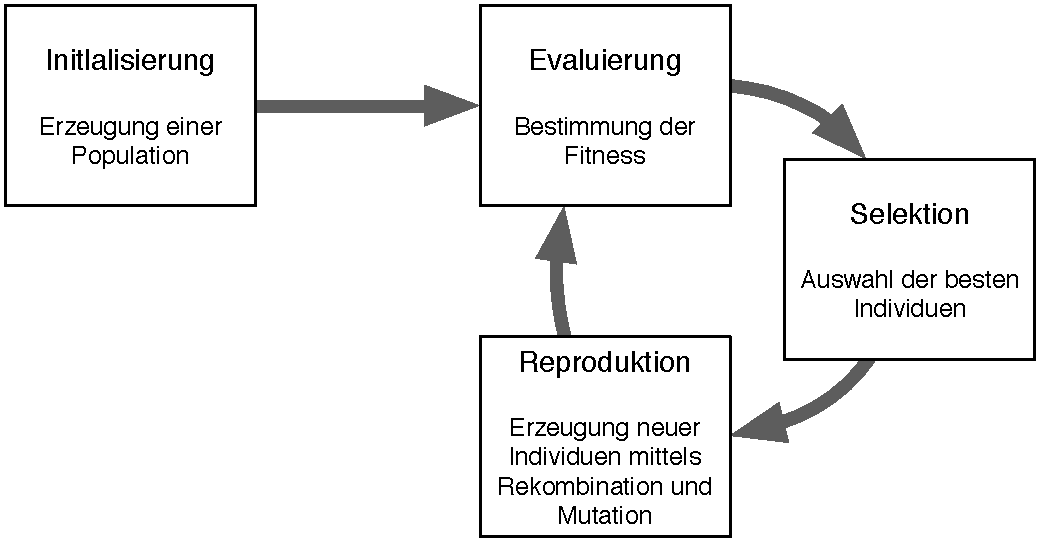
\includegraphics[width=0.8\textwidth]{evo_basic}
\caption{Ablauf evolutionärer Algorithmen}
\label{fig:evo_basic}
\end{figure}

Die einzelnen Komponenten eines evolutionären Algorithmus werden im Folgenden beschrieben. Die Definitionen folgen dabei im Wesentlichen denen von \textcite{tw2008}.

\paragraph{Initialisierung}

Die Population \(P\) stellt eine Menge von Lösungskandidaten dar. Ein Lösungskandidat \(i\) wird dabei als \emph{Individuum} bezeichnet und durch seinen \emph{Genotyp} repräsentiert. Der Genotyp ist die kodierte Repräsentation aller Variablen, die den Lösungskandidaten spezifizieren. Die Variablen werden \emph{Gene} genannt. Im Initlaisierungsschritt werden Lösungskandidaten erzeugt, die die Startpopulation des evolutionären Algorithmus bilden. Die Gene jedes Individuums werden dabei üblicherweise zufällig gewählt.

\paragraph{Evaluierung}

Der Evaluierungsschritt dient zur Bestimmung der \emph{Fitness} der Individuen, die noch in der Population enthalten sind. Die Fitness stellt dabei einen Wert dar, der die Güte der durch das Individuum repräsentierten Lösung bezüglich der Problemstellung beschreibt. Die Fitness kann dabei, je nach Optimierungsproblem, entweder absolut oder bezüglich der anderen Individuen der Population bestimmt werden. Somit lässt sich die Funktion zur Bestimmung der Fitness auf die Form \(fitness(i, P)\) generalisieren.

\paragraph{Selektion}

Im Selektionsschritt werden die fittesten Individuen der Population ausgewählt. Alle nicht ausgewählten Lösungskandidaten werden verworfen. Die Selektion kann dabei als Funktion der Form \(select(P, f, s)\) dargestellt werden, wobei \(s\) eine festgelegte Anzahl von Individuen darstellt, die ausgewählt werden sollen.

\paragraph{Reproduktion}

Die Reproduktion dient dazu, aus den im Selektionschritt ausgewählten Individuen neue Lösungskandidaten zu erzeugen. Dabei werden üblicherweise die Operationen \emph{Rekombination} und \emph{Mutation} verwendet. Eine Rekombination erzeugt dabei, analog zur Biologie, aus zwei Elternindividuen ein neues Kindindividuum. Sie lässt sich dabei als Funktion der Form \(i_n = recombine(i_a, i_b)\) darstellen, wobei \(i_n\) das neue Individuum und \(i_a\) und \(i_b\) die Elternindividuen darstellen. Eine Mutation erzeugt ein neues Individuen durch die Modifikation eines anderen und ist daher durch die Funktion \(i_n = mutate(i_a)\) spezifiziert.

In der Literatur \cite{kw2007, tw2008, dj2006} finden sich für Selektion, Mutation und Rekombination Standardverfahren, die in Hinblick auf das zu lösende Optimierungsproblem ausgewählt werden können. Wie die beschriebenen Schritte des evolutionären Algorithmus für die Optimierung der Link Discovery implementiert wurden, wird im folgenden Abschnitt beschrieben.

\section{Umsetzung}

Nachdem im vorhergehenden Abschnitt die Grundlagen und Komponenten evolutionärer Algorithmen beschrieben wurden, werden im Folgenden die für die Optimierung der Link Discovery-Ergebnnise angewendeten Methoden erläutert.

Zunächst soll die Methode zur Auswahl der Stichproben erläutert werden. Insgesamt wurden fünfzehn Knoten ausgewählt, deren Beziehungen optimiert werden sollen. Die Auswahl der Knoten richtete sich dabei nach der Popularität von Suchbegriffen auf der Spreadshirt-Plattform. Dazu wurden alle Begriffe mit mehr als eintausend Suchen herangezogen und diese nach Häufigkeit der Suchen geordnet. Daraus wurden zufällig je fünf Begriffe bis zum unteren Quartil, fünf Begriffe zwischen unterem und oberen Quartil und fünf Begriffe über dem oberen Quartil ausgewählt. Die ausgewählten Begriffe, deren Kantengewichtungen lokal optimiert werden sollen, lauten: \emph{Kopfkissenbezug}, \emph{Student}, \emph{Volkswagen}, \emph{Marathon}, \emph{Wow}, \emph{Krankenschwester}, \emph{Mountainbike}, \emph{Hammer}, \emph{Polska}, \emph{Regenbogen}, \emph{Minecraft}, \emph{Kind}, \emph{Dubstep}, \emph{Leipzig} und \emph{Valentinstag}.

Ziel dieser Auswahl war, eine möglichst vielfältige Verteilung der einzelnen Kantentypen zu erreichen, aus welcher sich nach Durchführung der Optimierung möglicherweise Erkenntnisse ableiten lassen, ob die Optimierung nur lokal oder auch global druchgeführt werden kann.

\section{Auswertung der Ergebnisse}
\chapter{Schlussbetrachtung}
\label{summary}

In dieser Masterarbeit wurde ein Verfahren und dessen praktische Durchführung zum Finden von Zusammenhängen zwischen Begriffen, die \emph{Link Discovery}, beschrieben. Die Basis dafür stellten die Daten eines Tagging--Systems dar. Dazu wurden Tagging--Systeme grundlegend erläutert, deren Datenmodell definiert und die grundlegenden Unterschiede zwischen Folksonomies und geschlossenen Tagging--Systemen herausgearbeitet. Die Eigenschaften des im späteren Verlauf verwendeten Tagging--Systems von Spreadshirt wurden beschrieben und dessen Datenqualität in Hinblick auf Korrektheit, Vollständigkeit und Redundanzfreiheit diskutiert. Außerdem wurden die zu verarbeitenden Datenmengen definiert.

Für die Durchführung der Link Discovery wurde ein Framework definiert, welches die konzeptionelle Grundlage für die spätere Umsetzung darstellt. Dieses Framework modelliert den betrachteten Weltausschnitt, welcher Begriffe, den Kontext von Begriffen und deren Beziehungen untereinander enthält. Dieser Weltausschnitt wurde in eine Graphenrepräsentation überführt. Weiterhin wurde der Prozess der Link Discovery definiert und die einzelnen Schritte erläutert. Diese bestehen in der initialen Erstellung des Weltausschnittes, der Anreicherung durch Mining oder Integration weiterer Datenquellen und der Priorisierung der erzeugten Beziehungen. Die theoretischen Grundlagen von Kookkurrenz zur Beziehungserzeugung wurden definiert und die Berechnung veranschaulicht.

Weiterhin wurden mögliche Datenquellen diskutiert und die für die praktische Durchführung der Link Discovery in dieser Arbeit verwendeten Quellen ausgewählt. Diese bestehen aus dem Tagging-- und Clicktracking--System von Spreadshirt sowie dem Wortschatz der Universität Leipzig. Zur Priorisierung der erzeugten Beziehungen wurden evolutionäre Algorithmen erläutert und deren Einsatz im Rahmen der Priorisierung definiert.

Diese theoretischen Grundlagen wurden anschließend an konkreten Daten praktisch umgesetzt. Für jede integrierte Datenquelle wurden die Schritte Import, Bereinigung, Reduktion, Transformation in die Graphenrepräsentation und Integration in den Weltausschnitt ausführlich dargestellt und die quantitativen Ergebnisse präsentiert. Zur Anreicherung durch Mining wurde die Zerlegung von Wortgruppen in Einzelwörter erläutert. Im Anschluss wurden die quantitativen Veränderungen der Graphenrepräsentation nach jedem Link--Discovery--Schritt dargestellt und diskutiert. Nachdem alle Datenquellen integriert waren, wurde die praktische Umsetzung der Priorisierung der Beziehung mittels evolutionärer Algorithmen dargestellt und die Ergebnisse präsentiert.

Weiterhin wurden die Anforderungen an ein technisches System, welches die Link Discovery implementiert, formuliert und deren Umsetzung im Rahmen dieser Arbeit beschrieben. Dazu gehören die Wahl des Datenbanksystems MongoDB, die Implementierung der Komponenten in der Programmiersprache JavaScript und die Beschreibung von Kookkurrenzberechnung mittels des Programmiermodells MapReduce.

Die Ergebnisse dieser Arbeit stellen die Grundlage für weitere mögliche Arbeiten dar. Eine zukünftige Arbeit könnte sich mit der Auswertung der inhaltlichen Qualität der erzeugten Beziehungen beschäftigen. Dazu wird eine gründliche Analyse der integrierten Datenquellen und des Ergebnisses der Link Discovery mit Hilfe menschlicher Beurteilung benötigt.

Weiterhin sind Arbeiten denkbar, die die erzeugten Beziehungen für weitere Analyseverfahren nutzen. So könnten beispielsweise die Beziehungen zum Clustering der Begriffe zu Themen genutzt werden. Werden hierarchische Clusteringverfahren genutzt, können daraus Themenbäume und Topic Maps abgeleitet werden. Diese Themenbäume können sich durch ständige Durchführung der Link Discovery an aktuelle Trends in den Inhalten der betrachteten Website anpassen.

Der Link--Discovery--Prozess könnte durch einen interaktiven Trainingsschritt erweitert werden. In diesem Schritt wird die Beurteilung der Beziehungen durch Benutzer nicht nur zur Priorisierung, sondern zur direkten Veränderung des Weltausschnittes genutzt. Dabei werden Kanten eingefügt, die explizite statt nachträglich hergestellte Zusammenhänge beschreiben. Außerdem könnten durch manuellen Eingriff fehlerhafte Beziehungen gelöscht werden.

Insgesamt stellt das in dieser Arbeit beschriebene Framework eine gute Basis für Erweiterungen und neue Implementierungen dar. Das Verfahren ist flexibel und leistungsfähig genug, um auch auf anderen Datenbeständen gute Ergebnisse erzielen zu können. Durch Integration anderer Datenquellen und neuer Analyseverfahren kann die Qualität der gefundenen Zusammenhänge stetig verbessert werden. Die konkret erzeugten Daten bieten eine gute Grundlage für weitere Auswertungen und praktische Anwendungen.

\listoffigures
\listoftables
\lstlistoflistings

\sloppy
\printbibliography 

\end{document}